%!TEX program = xelatex
\documentclass[dvipsnames, svgnames,a4paper,11pt]{article}
% ----------------------------------------------------
%   中山大学物理与天文学院本科实验报告模板
%   作者:Huanyu Shi,2019级
%   知乎:https://www.zhihu.com/people/za-ran-zhu-fu-liu-xing
%   Github:https://github.com/huanyushi/SYSU-SPA-Labreport-Template
%   Last update : 2023.4.10
% ----------------------------------------------------

% ----------------------------------------------------- 
%	加边框的命令
%	参考:https://tex.stackexchange.com/questions/531559/how-to-add-the-page-border-for-first-two-pages-in-latex
\usepackage{tikz}
\usetikzlibrary{calc}
\usepackage{eso-pic}
\AddToShipoutPictureBG{%
\begin{tikzpicture}[overlay,remember picture]
\draw[line width=0.6pt] % 边框粗细
    ($ (current page.north west) + (0.6cm,-0.6cm) $)
    rectangle
    ($ (current page.south east) + (-0.6cm,0.6cm) $); % 边框位置
\end{tikzpicture}}


\usepackage{xcolor}
\definecolor{c1}{HTML}{2752C9} % 目录颜色
\definecolor{c2}{RGB}{190,20,83} % 引用颜色

\usepackage{ctex}
\usepackage[top=28mm,bottom=28mm,left=15mm,right=15mm]{geometry}
\usepackage{hyperref} 
\hypersetup{
	colorlinks,
	linktoc = section, % 超链接位置,选项有section, page, all
	linkcolor = c1, % linkcolor 目录颜色
	citecolor = c1  % citecolor 引用颜色
}
\usepackage{amsmath,enumerate,multirow,float}
\usepackage{tabularx}
\usepackage{tabu}
\usepackage{subfig}
\usepackage{fancyhdr}
\usepackage{graphicx}
\usepackage{wrapfig}  
\usepackage{physics}
\usepackage{appendix}
\usepackage{amsfonts}

%
\usepackage{tcolorbox}
\tcbuselibrary{skins,breakable}
\newtcolorbox{tbox}[2][]{
    colframe=black!70!,
    breakable,
    enhanced,
	boxrule =0.5pt,
    title = {#2},
    fonttitle = \large\kaishu\bfseries,
	drop fuzzy shadow,
    #1
}
\newtcolorbox[auto counter,number within=section]{question}[1][]{
  top=2pt,bottom=2pt,arc=1mm,
  boxrule=0.5pt,
%   frame hidden,
  breakable,
  enhanced, %跨页后不会显示下边框
  coltitle=c1!80!gray,
  colframe=c1,
  colback=c1!3!white,
  drop fuzzy shadow,
  title={思考题~\thetcbcounter:\quad},
  fonttitle=\bfseries,
  attach title to upper,
  #1
}

% ---------------------------------------------------------------------
%	利用cleveref改变引用格式,\cref是引用命令
\usepackage{cleveref}
\crefformat{figure}{#2{\textcolor{c2}{图 #1}}#3} % 图片的引用格式
\crefformat{equation}{#2{(\textcolor{c2}{#1})}#3} % 公式的引用格式
\crefformat{table}{#2{\textcolor{c2}{表 #1}}#3} % 表格的引用格式


% ---------------------------------------------------------------------
%	页眉页脚设置
\fancypagestyle{plain}{\pagestyle{fancy}}
\pagestyle{fancy}
\lhead{\kaishu 中山大学物理与天文学院近代物理实验\uppercase\expandafter{\romannumeral1}} % 左边页眉,学院 + 课程
\rhead{\kaishu D4-1 \quad 电子自旋共振实验} % 右边页眉,实验报告标题
\cfoot{\thepage} % 页脚,中间添加页码


% ---------------------------------------------------------------------
%	对目录、章节标题的设置
\renewcommand{\contentsname}{\centerline{\huge 目录}}
\usepackage{titlesec}
\usepackage{titletoc}
% \titleformat{章节}[形状]{格式}{标题序号}{序号与标题间距}{标题前命令}[标题后命令]
\titleformat{\section}{\centering\LARGE\songti}{}{1em}{}

% ---------------------------------------------------------------------
%   listing代码环境设置
\usepackage{listings}
\lstloadlanguages{python}
\lstdefinestyle{pythonstyle}{
backgroundcolor=\color{gray!5},
language=python,
frameround=tftt,
frame=shadowbox, 
keepspaces=true,
breaklines,
columns=spaceflexible,                   
basicstyle=\ttfamily\small, % 基本文本设置,字体为teletype,大小为scriptsize
keywordstyle=[1]\color{c1}\bfseries, 
keywordstyle=[2]\color{Red!70!black},   
stringstyle=\color{Purple},       
showstringspaces=false,
commentstyle=\ttfamily\scriptsize\color{green!40!black},%注释文本设置,字体为sf,大小为smaller
tabsize=2,
morekeywords={as},
morekeywords=[2]{np, plt, sp},
numbers=left, % 代码行数
numberstyle=\it\tiny\color{gray}, % 代码行数的数字字体设置
stepnumber=1,
rulesepcolor=\color{gray!30!white}
}




% ---------------------------------------------------------------------
%	其他设置
\def\degree{${}^{\circ}$} % 角度
\graphicspath{{./images/}} % 插入图片的相对路径
\allowdisplaybreaks[4]  %允许公式跨页 % 导入模板的相关设置
\usepackage{lipsum}
\usepackage{enumitem}
\usepackage{tabularray}  %绘制表格时可以更加方便添加框线
\usepackage{titling} % 引入titling宏包
% \usepackage{subcaption}
\usepackage{wrapfig}
\usepackage{longtable}
\usepackage{listings}
\usepackage{xcolor}


\setlist[enumerate]{label=\textup{(\arabic*)}}





% \title{热力学第二定律设计性实验}
% \pretitle{\begin{center}\LARGE\bfseries}
% \posttitle{\par\end{center}\vskip 0.5em}

% \preauthor{}
% \postauthor{}

% \author{
%     \begin{center}
%         \begin{tabular}{ll}
%             \underline{戴鹏辉} & 学号:\underline{22344016} \\
%             姓名:\underline{杨舒云} & 学号:\underline{22344020}
%         \end{tabular}
%     \end{center}
% }

% \date{}

% % 自定义命令用于插入副标题
% \newcommand{\   subtitle}[1]{%
%     \begin{center}\large#1\end{center}%
%     \vskip 1em
% }

%---------------------------------------------------------------------
%	正文
%---------------------------------------------------------------------

\begin{document}

\begin{center}
    {\Huge \textbf{热力学第二定律设计性实验}} \\
    \bigskip
    {\Large \textbf{基于热电效应的热机设计与热力学第二定律验证实验}}

\end{center}

\begin{table}[htbp]
    \centering
    \begin{tblr}{
    }
    姓名: & \underline{戴鹏辉} & 学号: & \underline{22344016} \\
    姓名: & \underline{杨舒云} & 学号: & \underline{22344020} 
    \end{tblr}
\end{table}

\section{摘要}

本实验旨在通过设计并验证一个基于热电效应的热机系统,以深入理解和验证热力学第二定律。热电效应包括Seebeck效应、Peltier效应和Thomson效应,这些效应在热机设计中起到关键作用。实验过程中,我们使用了热电模块(TEC片)、加热电阻、冷却系统、导热铜片、外电路和散热风扇,搭建了实验装置,并进行了系统的测量和分析。

在实验的初始阶段,我们通过固定冷热端温差,测量热机的外负载特性。通过调整负载电阻,获取不同负载条件下的输出电压和电流,并基于这些数据计算出热电发电装置的电动势和内阻。实验结果显示,热电发电装置的最大输出功率出现在负载电阻与内阻相等时。
随后,我们进行了Seebeck系数的测量。通过控制热端和冷端的温度差异,建立稳定的温差,并测量热电材料两端的开路电压,从而计算出Seebeck系数。实验结果显示,Seebeck系数与温差成线性关系,这与理论预期一致。

为了进一步优化热机的性能,我们分析了TEC内阻随温差变化的情况,并研究了双TEC耦合热电堆的性能。通过将多个TEC片串联或并联,我们探索了不同耦合方式对输出电压、电流和功率的影响。结果表明,合适的耦合方式可以显著提高热电发电装置的输出性能。
在实验的最后阶段,我们基于热力学原理进行了散热特性的建模分析。通过计算对流和辐射散热,评估了热机在不同温差条件下的散热情况。结果显示,优化热源和冷源的温度可以有效减少散热损失,从而提高热机效率。

综合以上实验结果,本研究成功验证了热力学第二定律,展示了基于热电效应的热机设计在能量转换中的潜力和挑战。实验过程中,测量误差的评估和控制也是一个关键环节,通过使用高精度的温度和电压测量设备,以及精确的温度控制系统,我们尽可能减少了外界因素对实验结果的影响。

总体而言,本实验不仅验证了热力学第二定律,还为未来基于热电效应的热机设计提供了重要的实验数据和理论基础。

\textbf{关键词:}热电效应,Seebeck效应,热机效率,热力学第二定律,能量转换,散热优化。


\clearpage
\tableofcontents
\clearpage









\section{背景介绍}

    \subsection{热力学第一定律与热力学第二定律}
        
        \begin{itemize}
            \item \textbf{热力学第一定律:}热力学第一定律,又称能量守恒定律,指出在一个孤立系统中,能量既不会凭空产生也不会凭空消失,只会从一种形式转化为另一种形式。这一定律表明了能量守恒的原理,即系统的总能量变化等于系统所吸收的热量与所做功的总和。用数学形式表示为:
            \[
            \Delta U = Q + W
            \]
            其中 $\Delta U$ 是系统内能的变化,$Q$ 系统是吸收的热量,$W$ 是外界对系统做的功。热力学第一定律奠定了热能与机械能之间的转换关系,是热机和其他能量转换装置设计的基础。
            

            \item \textbf{热力学第二定律:}热力学第二定律描述了自然界中能量转移的方向性和不可逆性,具体表述为克劳修斯表述和开尔文表述。

                \begin{itemize}
                    \item \textbf{克劳修斯表述:}
                    \begin{enumerate}
                        \item 热力学第二定律的克劳修斯表述指出,不可能将热量从低温物体自发地传递给高温物体,而不引起其他变化。
                        \item 这表明了热量传递的方向性,即热量不会自发地从冷物体流向热物体。
                    \end{enumerate}
                    
                    \item \textbf{开尔文表述:}
                    \begin{enumerate}
                        \item 另一种表述是开尔文表述,它指出不可能从单一热源吸热使之完全转化为功而不产生其他影响。
                        \item 这个表述强调了能量转化过程中不可避免的能量损耗或者其他形式的能量转移。
                    \end{enumerate}
                \end{itemize}

            

                
        
        \end{itemize}



    
    \subsection{热机}

        \begin{itemize}
            \item \textbf{热机的基本原理:}热机的基本工作原理基于热力学定律,特别是热力学第一定律(能量守恒定律)和第二定律(熵增原理)。简单来说,热机利用高温热源和低温热汇之间的温差,通过一定的循环过程将部分热能转化为机械能或电能,而未转化的部分热能则被低温热汇吸收。\textbf{热电发电机}则利用塞贝克效应(Seebeck Effect)将热能直接转化为电能。
            
            \item \textbf{热电发电机的优缺点:}热电发电机具有无运动部件、静音运行、模块化设计和多种热源适应性的优点,因此它具有高可靠性、低维护需求、易于集成和扩展,并能够利用太阳能、地热、废热等多种形式的热源。然而,它也存在能量转换效率较低(一般在5\%到10\%之间)和成本较高的缺点,这些限制了其大规模应用。通过材料研究和制造工艺的改进,未来有望提升效率并降低成本,使其在更多领域得到广泛应用。
            
            \item \textbf{卡诺循环:}卡诺循环是理想热机循环的理论模型,由法国物理学家萨迪·卡诺在1824年提出。卡诺循环包括两个等温过程和两个绝热过程,通过对高温热源吸热、对低温热源放热,实现能量转换。卡诺定理指出,任何实际热机的效率都不可能超过卡诺热机的效率,这为热机设计提供了理论上限。
            
            \item \textbf{量子热机:}现代热机的研究不仅限于宏观尺度,还扩展到了微观和量子尺度。例如,量子热机在近年来引起了广泛关注。研究表明,量子热机在某些条件下可以超越传统的卡诺效率,这主要得益于量子力学效应带来的新特性。尽管如此,量子热机仍需遵循热力学第二定律,只不过其效率上限受制于量子效应。


        \end{itemize}
















\section{基本原理与实验方案}
    
    
    \subsection{基本原理}

        \begin{enumerate}
            \item \textbf{热电效应:}
            
                \begin{figure}[htbp]
                    \centering
                    \subfloat[Seebeck效应原理图]{
                        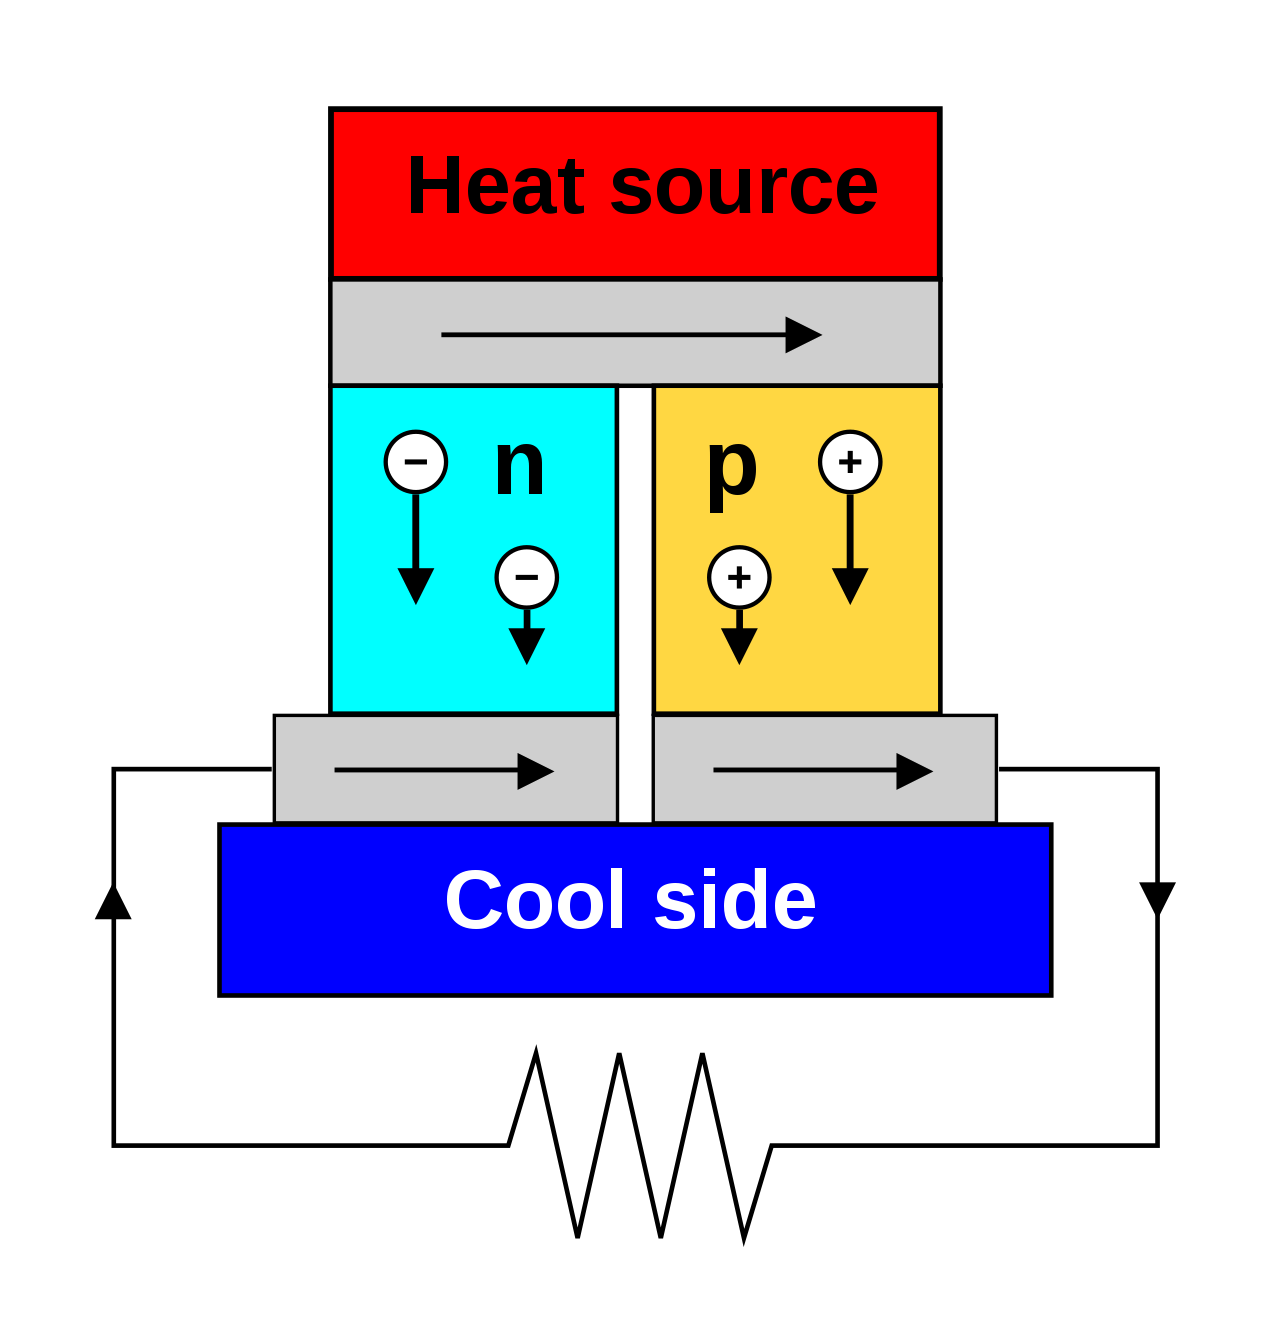
\includegraphics[width=0.4\textwidth]{SamPre_1_Gra3.png}
                    }
                    \subfloat[Peltier效应原理图]{
                        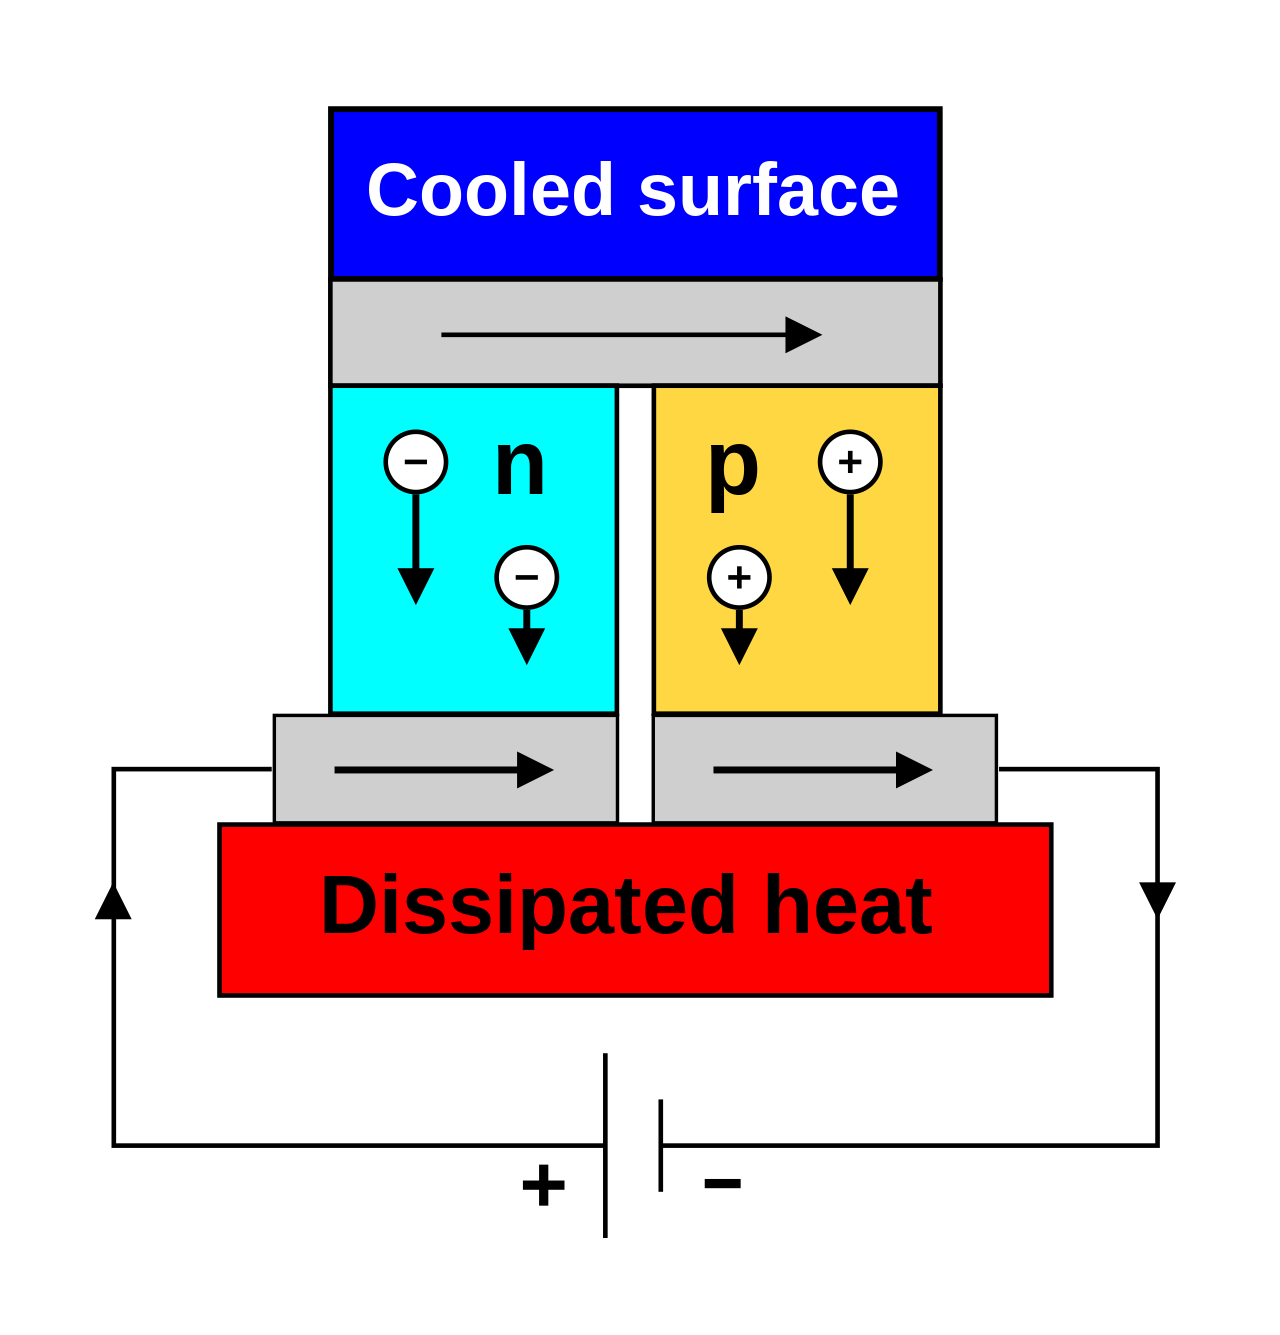
\includegraphics[width=0.4\textwidth]{SamPre_1_Gra4.png}
                    }	
                \end{figure}

                \begin{itemize}
                    \item Seebeck 效应:当两种不同的导体或半导体连接成回路,并且两个接头的温度不同,就会在回路中产生\textbf{电动势}
                    
                        \[
                            \mathrm{d}V=\epsilon_{AB}\mathrm{d}T
                        \]
                        其中,$\epsilon_{AB}$是温差电动势系数(又称\textbf{Seebeck系数},记为$\alpha$)。符号约定为如果在高温段电动势驱使电流由金属A流向金属B为正。
        P
                    \item Peltier效应: 当电流通过两种不同材料组成的电路时,一个接头会吸热,另一个接头会放热。
                    
                        \[
                            \textbf{J}_{q\pi}=\pi_{AB}\textbf{J}_{e}
                        \]
        
                        其中,$\textbf{J}_{q\pi}$是Peltier热流密度,$\textbf{J}_{e}$是从A到B的电流密度,$\pi_{AB}$是两种金属的Peltier系数(与温度有关)。
        
                    \item Thomson效应:在均质导体中,如果存在温度梯度,当电流通过时,会伴随着吸热或放热的现象。这对于完整的热电模型和效率分析很关键。$\dot{Q}=\mu I\cdot \nabla T$,$\mu$为Thomson系数。
        



                \end{itemize}




            \item \textbf{Seebeck效应电源的外输出特性:}
            

                
                \begin{itemize}
                    \item 开路电压是指没有外部负载连接时,热电发电装置两端的电压。根据Seebeck效应,开路电压与温差成正比,$V_{\text{oc}} = \alpha \Delta T$。
                    
                    \item 当热电发电装置连接到负载时,输出电压会由于内阻的存在而下降。负载电压$V_{\text{L}} = \frac{\alpha \Delta T \cdot R_{\text{L}}}{R_{\text{L}} + R_{\text{in}}}$,而输出功率是负载上消耗的功率$P_{\text{out}} = \frac{(\alpha \Delta T)^2 \cdot R_{\text{L}}}{(R_{\text{L}} + R_{\text{in}})^2}$。
                    
                    \item \textbf{当负载电阻等于内阻时},热电发电装置输出的功率达到最大$P_{\text{max}} = \frac{(\alpha \Delta T)^2}{4 R_{\text{in}}}$。				
                \end{itemize}


            \item \textbf{热力学建模}
            \begin{itemize}
                \item Newton冷却定律:
                \[
                Q_{\text{conv}} = h A (T_{\text{surface}} - T_{\text{ambient}})
                \]
                其中 \( h \) 是对流换热系数, \( A \) 是热机的表面积, \( T_{\text{surface}} \) 是热机的表面温度, \( T_{\text{ambient}} \) 是环境温度。
                
                \item Stefan-Boltzmann定律:
                \[
                Q_{\text{rad}} = \epsilon \sigma A (T_{\text{surface}}^4 - T_{\text{ambient}}^4)
                \]
                其中 \( \epsilon \) 是热机表面的发射率, \( \sigma \) 是Stefan-Boltzmann常数, \( A \) 是热机的表面积, \( T_{\text{surface}} \) 和 \( T_{\text{ambient}} \) 分别是热机表面温度和环境温度。
            \end{itemize}

      \end{enumerate}








    \subsection{实验方案}
    
        % \begin{enumerate}
        %     \item 各元件性能测量
        %     \begin{itemize}
        %         \item \textbf{Seebeck效应测量}:通过改变温差并测量开路电压来研究Seebeck效应,从而确定$\alpha$;
        %         \item 器件内阻的测量与影响:内阻对热电转换效率有重要影响,了解并优化内阻对提高热机性能是必要的;
        %         \item 考虑测量电加热器的加热功率(以及其它元件性能,如Peltier效应)。
        %     \end{itemize}
            
        %     \item 搭建热机
        %         \begin{itemize}
        %             \item \textbf{热电堆集成——电加热器与Seebeck元件,测控部分——PID控温(热端、冷端),输出电路部分(输出功率测量)。}
        %         \end{itemize}
            
        %     \item 负载与效率测量
        %     \begin{itemize}
        %         \item \textbf{加热功率测控}——电流表电压表实时测控(含于PID系统中,编写相关程序);
        %         \item \textbf{输出功率测控}——电流表电压表实时测控(考虑是否编程);
        %         \item 测量最大输出功率——改变输出电路的负载;
        %         \item 测量最大输出效率——改变温差与负载,优化其它部分;
        %         \item 探究如何测量热端的损失。
        %     \end{itemize}
            
        %     \item 热力学第二定律的展示
        %     \begin{itemize}
        %         \item \textbf{通过实验测量,展示即使是优化过的热电装置,其效率也受到卡诺效率的限制,这直接体现了热力学第二定律。}
        %         \item 讨论如何通过实验设计来逼近卡诺效率,包括使用最佳材料、最佳温差和最佳负载条件。
        %     \end{itemize}			
            
        %     \item 结论与进一步的探索
        %     \begin{itemize}
        %         \item 比较热机效率与理论卡诺效率的差异,讨论可能的优化途径和技术挑战;
        %         \item 探究各部分如何\textbf{优化}(热电堆——减小散热,增大温差,冷热端优化;测控——优化控温算法,改进实时测量程序;输出电路部分——减小散热,考虑Thomson效应的影响;理论建模——估算散热进一步修正)。
        %     \end{itemize}
        % \end{enumerate}


        \begin{itemize}
            \item \textbf{器件内阻的测量与影响}
            
                当TEC片的冷、热端温差恒定时,可视为其电动势恒定。将热机等效为一个电动势$E$加一个内阻$R_s$,电路图如\cref{fig:电路图}所示。所接的外负载是一个滑动变阻器。由电路方程
                \[
                    U_L = E - I \cdot R_L
                \]
                可知,只需改变电路的外负载,即可得到$U_L - I$的关系。再对实验数据用该电路方程进行线性拟合,即可得到热机的电动势$E$和内阻$R_s$。

                \begin{figure}[htbp]
                    \centering
                    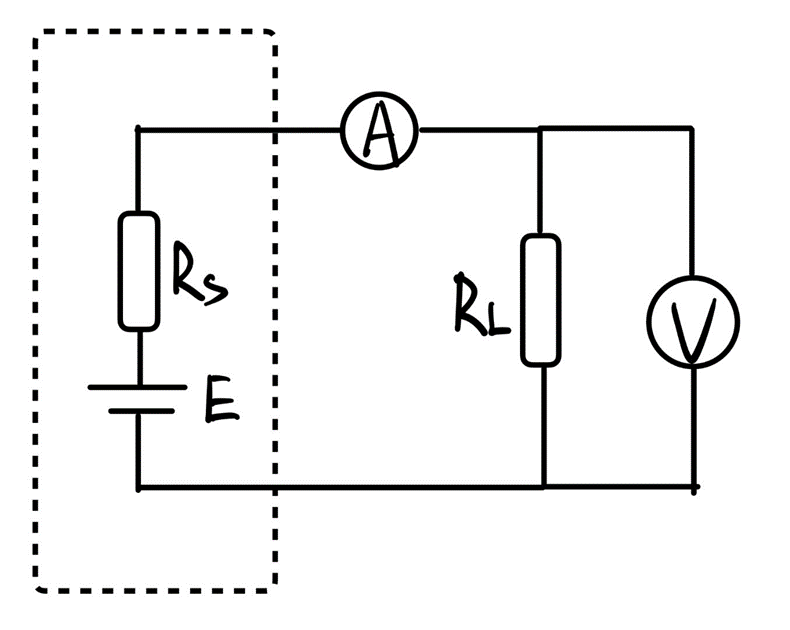
\includegraphics[width=0.35\textwidth]{电路图.png}
                    \caption{热机外负载特性电路图}
                    \label{fig:电路图}
                \end{figure}

            \item \textbf{Seebeck效应测量}
            

                Seebeck效应的测量过程如下:

                \begin{enumerate}
                    \item 实验装置的准备:搭建一个包含热端和冷端的热电材料实验装置。热端通过电加热器加热,冷端通过冷却设备(如风扇或散热器)冷却。
                    \item 温差的建立:通过控制热端和冷端的温度,建立一个稳定的温差。使用PT100温度传感器分别测量热端和冷端的温度。
                    \item 电压测量:在温差建立后,使用高精度电压表测量热电材料两端的开路电压。
                    \item 数据记录与分析:记录不同温差下的开路电压值,并根据Seebeck效应公式
                    \[
                    \alpha = \frac{\Delta V}{\Delta T}
                    \]
                    计算热电材料的Seebeck系数$\alpha$。
                \end{enumerate}

            \item \textbf{热机整体规划}:详见\textbf{实验仪器搭建部分}。
            
            \item \textbf{效率优化:}
        
            \begin{enumerate}
                \item \textbf{增大注入系统的能量,减小散热}
                
                    通过增大热源温度$T_H$来增加注入系统的热量,同时降低冷源温度$T_C$以减少散出的热量,从而提高效率。具体措施包括选择更高温的燃料或改进燃烧技术,使用更高效的冷却技术或材料,采用高导热性材料减少热损失,优化热机的设计以减少内部摩擦和热损耗,加强系统的隔热性以减少热量流失,提高热交换器的效率,优化操作条件如压力和流速,并定期维护热机设备确保其在最佳状态下运行。

                \item \textbf{输入功率恒定,增大温差}
                
                    在输入功率保持不变的情况下,通过增加热源温度$T_H$和降低冷源温度$T_C$来增大温差,从而提高效率。具体措施包括采用高温材料、改进燃烧技术或使用高效能燃料如天然气或氢气,改进冷却系统使用更高效的冷却液或低温冷却剂,优化热交换系统提高热交换器效率,使用高导热材料和改进换热器设计,改进系统绝热性采用先进隔热材料和技术,采用多级加热和冷却技术逐步提高热源温度和降低冷源温度,以及使用精确的温度控制系统确保热源和冷源温度始终在最佳范围内。

                    \begin{figure}[htbp]
                        \centering
                        \subfloat[]{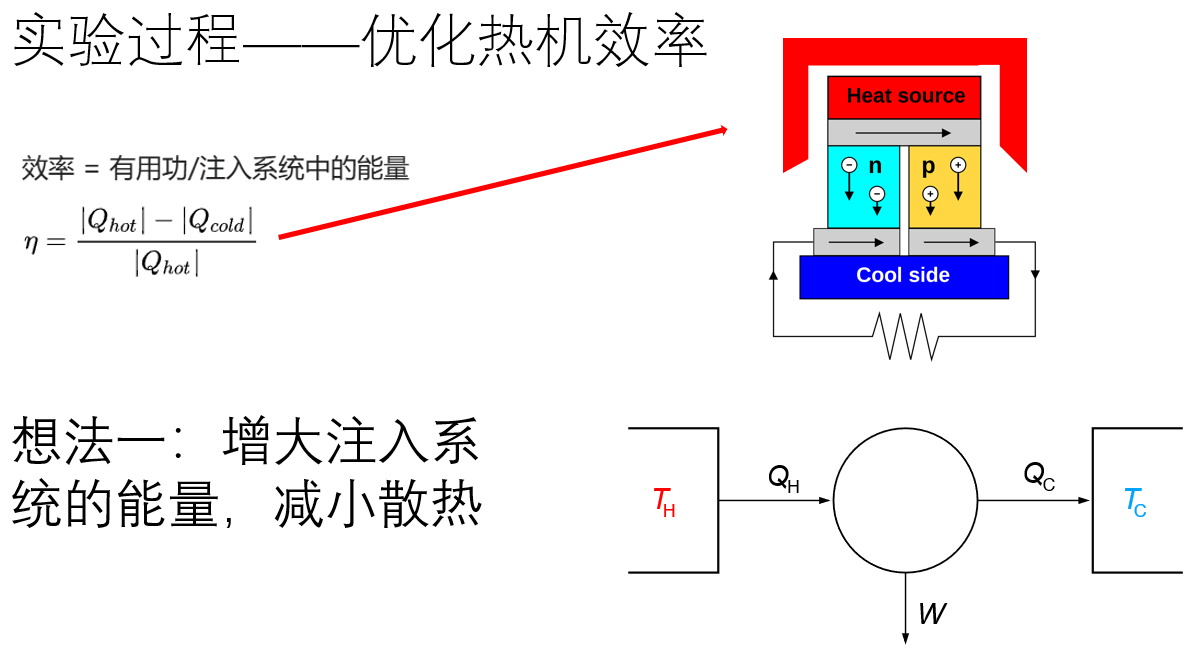
\includegraphics[width=0.3\textwidth]{热机效率优化1.png}\label{fig:热机效率优化1}}
                        \subfloat[]{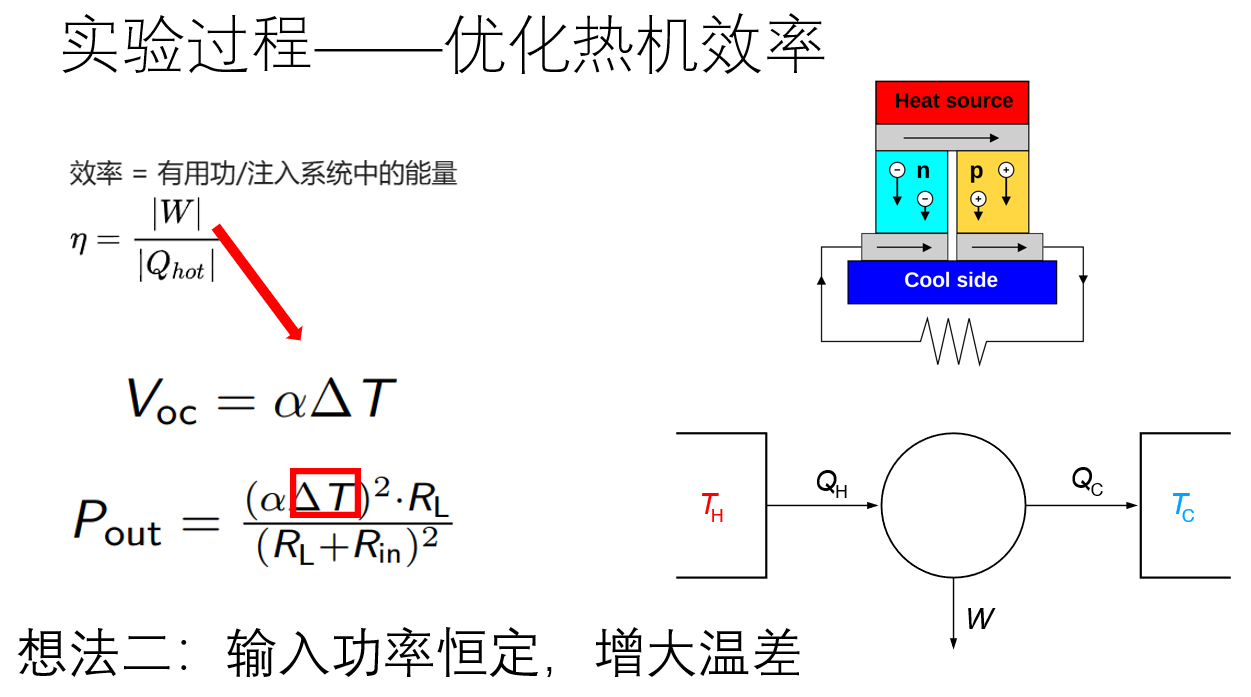
\includegraphics[width=0.3\textwidth]{热机效率优化2.png}\label{fig:热机效率优化2}}
                        \caption{}
                        \label{fig:热机效率优化}
                    \end{figure}

            \end{enumerate}
            
            \clearpage
            \item \textbf{热电堆的集成:}
            \begin{figure}[htbp]
                \centering
                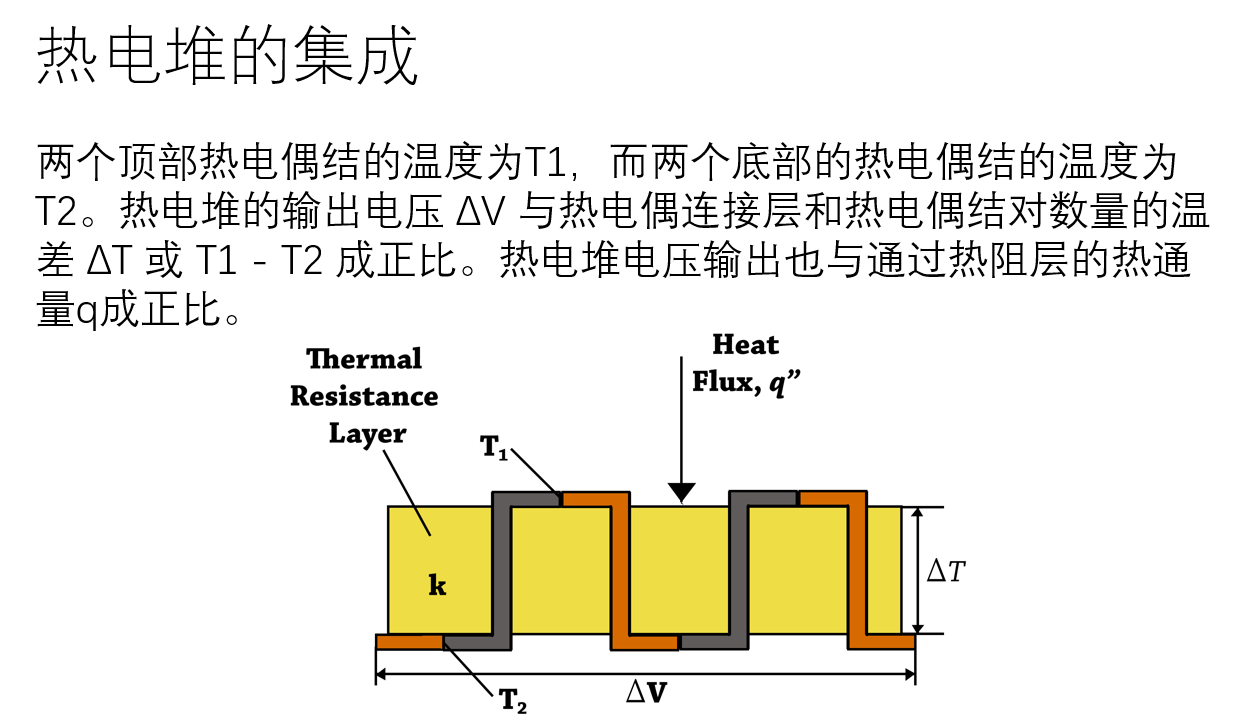
\includegraphics[width=0.8\textwidth]{热电堆的集成1.png}
            \end{figure}
            \begin{figure}[htbp]
                \centering
                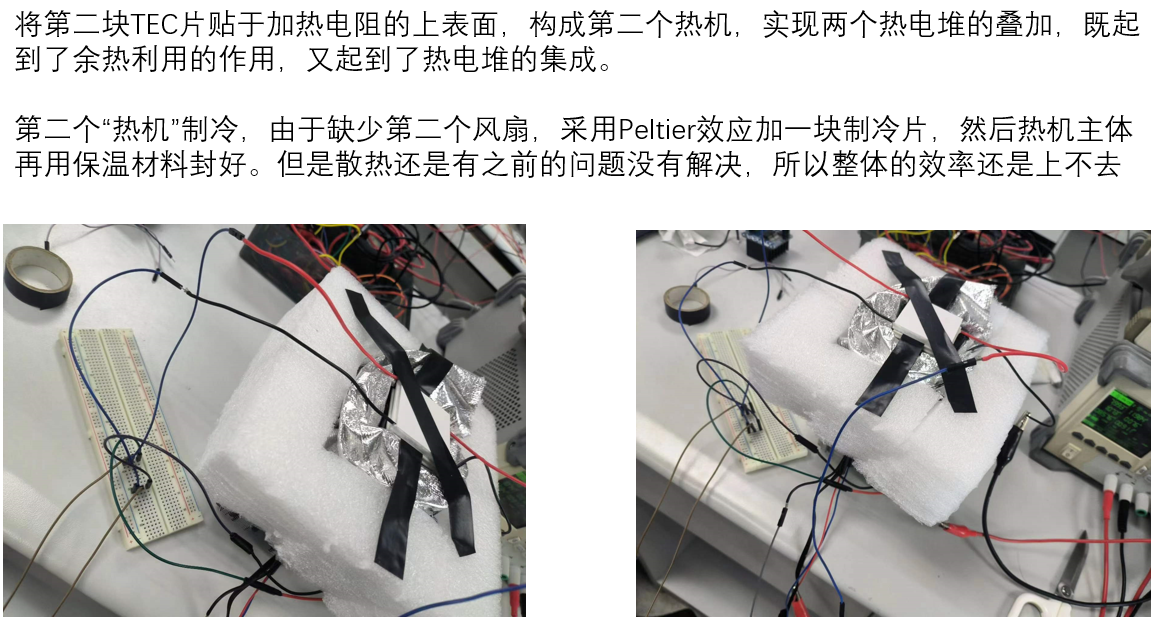
\includegraphics[width=0.8\textwidth]{热电堆的集成2.png}
            \end{figure}


            
        \end{itemize}


    \subsection{测量方程}

        \begin{itemize}
            \item \textbf{测温:}本实验测温使用PT100测温电阻,通过测量其电阻值得到温度,电阻与温度的关系为:
                \[
                    t = \frac{R_t(\Omega) - 100}{0.385} (℃)
                \]



            \item \textbf{输入功率:}
            
			    加热电阻丝直接使用直流稳压电源供电,通过读取电源上的电压和电流值,可以得到输入功率$P_{in} = U \cdot I$
			




            \item \textbf{输出功率:}
            
                \begin{itemize}
                    \item 当热电发电装置连接到负载时,负载电压$U_{\text{L}} = \frac{\alpha \Delta T \cdot R_{\text{L}}}{R_{\text{L}} + R_{\text{s}}}$,而输出功率是负载上消耗的功率$P_{\text{out}} = \frac{(\alpha \Delta T)^2 \cdot R_{\text{L}}}{(R_{\text{L}} + R_{\text{s}})^2}$。
                    
                    \item \textbf{当负载电阻等于内阻时},热电发电装置输出的功率达到最大$P_{\text{max}} = \frac{(\alpha \Delta T)^2}{4 R_{\text{s}}}$。	
                    
                \end{itemize}		








            \item \textbf{热机效率:}
            
                效率可通过热机对外做功$W$和吸热$Q$之比计算。
                \[
                    \eta = \frac{W}{Q_H} = \frac{U_L \cdot I_{out} \cdot t}{U_{in} \cdot I_{in} \cdot t} = \frac{U_L \cdot I_{out}}{U_{in} \cdot I_{in} } = \frac{P_{out}}{P_{in}}
                \]
            
        \end{itemize}



    \subsection{误差分配与可行性讨论}


        在基于热电效应的热机设计与热力学第二定律验证实验中,测量误差分配和可行性评估是关键的环节。首先,温度测量误差主要来源于PT100温度传感器的精度以及测温电桥的精度和分辨率。通常,PT100传感器的精度为±0.1℃,加上电桥的误差为±0.05℃,综合误差约为±0.11℃。其次,电压测量误差来自高精度电压表的测量误差和内阻影响。假设电压表的精度为读数的±0.1\%加上固定误差±0.01V,例如测量1V时,误差为±0.011V。电流测量误差类似,假设电流表的精度为读数的±0.2\%加上固定误差±0.01A,例如测量1A时,误差为±0.012A。

        输入功率的计算误差则来自电压和电流测量的综合误差。假设电压为12V,电流为2A,输入功率为24W,综合误差约为±0.264W。输出功率的计算误差也类似于输入功率的误差计算方法。这些测量误差将对实验结果产生影响,例如温度测量的误差会直接影响Seebeck系数的计算精度,而电压和电流的测量误差则会影响输入功率和输出功率的计算,从而影响热机效率的计算。
        
        在评估实验可行性时,需要综合考虑温差的建立与控制、测量设备的精度和实验环境的影响。为了保证温差的稳定,可以使用高精度的温控设备和优质的导热材料,通过PID控制器精确调节温度,减少温度波动带来的误差。使用高精度的测量仪器,例如高精度电压表和电流表,并定期校准传感器和测量仪器,以确保测量结果的准确性。实验环境也需控制好温度和湿度,减少外界环境变化对实验结果的干扰。使用绝缘材料减少热损失,确保测量数据的可靠性。
    



\clearpage
\section{实验装置搭建}


    \begin{figure}[htbp]
        \centering
        \subfloat[热机示意图]{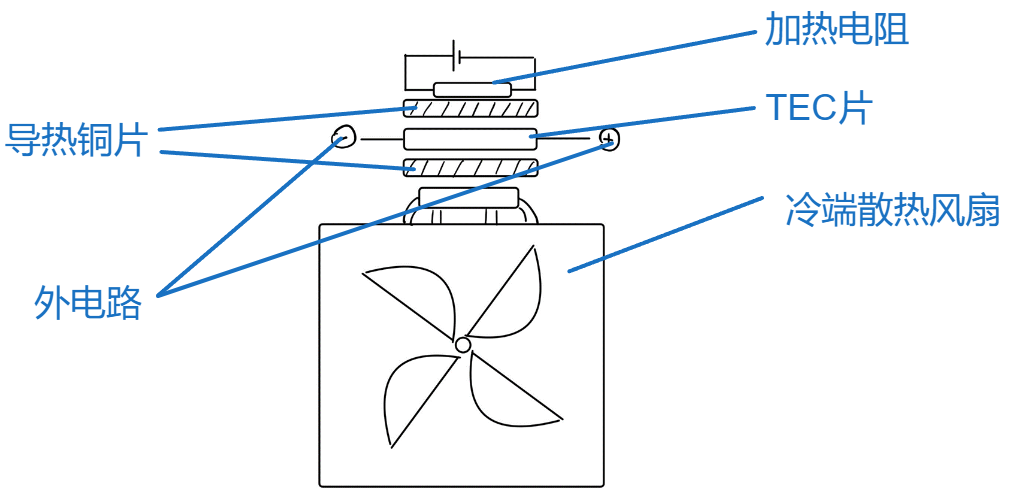
\includegraphics[width=0.8\textwidth]{热机示意图2.png}\label{fig:热机示意图2}}
        % \hfill
        % \subfloat[热机实物图]{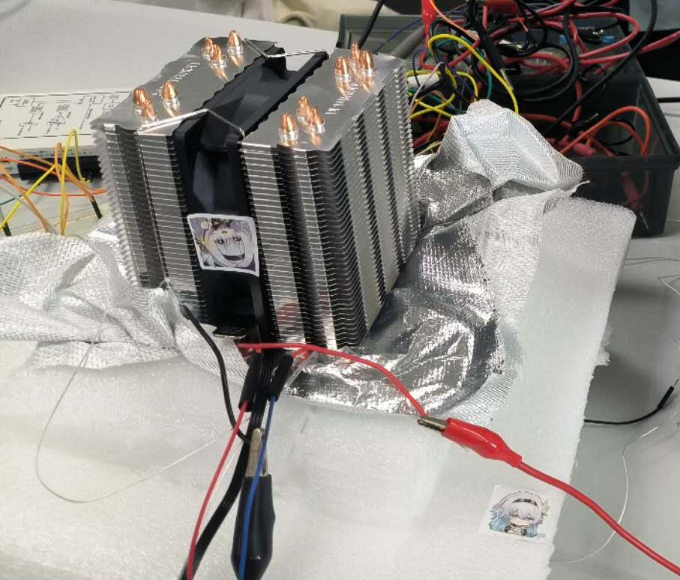
\includegraphics[width=0.4\textwidth]{热机实物图.png}\label{fig:热机实物图}}
        % \caption{热机}
        \label{fig:热机}
    \end{figure}

    \begin{itemize}
        \item \textbf{热机设计:}
            如\cref{fig:热机示意图2}所示,我们搭建了一个基于热电效应的热机实验装置。该装置包括热电模块(TEC片)、加热电阻、冷却系统、导热铜片、外电路和散热风扇。我们通过串联若干热电模块来增加输出电压,并根据所需的输出功率和单个热电模块的性能,计算所需的模块数量。如果需要增加输出电流,则可以将热电模块并联。

            实验装置的热源部分是通过将加热电阻固定在热电模块的一侧来实现的,确保热端能够获得足够高的温度。热电模块的另一侧安装了冷却系统,包括冷端散热风扇,以保持冷端的温度尽可能低,从而增加热电模块的温差。

            在电气连接方面,我们将电压表和电流表分别并联和串联到热电模块或模块组合的输出端,以便测量输出电压和电流。同时,将负载连接到热电模块的输出端,初始使用一个较高的电阻值作为基准。在测量过程中,我们逐步调整负载电阻,测量不同负载条件下的输出功率,找到输出功率最大时的负载电阻值,并记录最优负载条件下的输出电压、电流和功率。

            为了确保实验的安全性和数据的准确性,我们在热端和冷端分别安装了温度传感器,实时监控温度,确保热端温度在安全范围内,且冷端不会过热。此外,使用绝缘材料和防护措施,确保操作者不会直接接触到高温部分。通过上述装置和实验步骤,我们可以研究热电效应,测量Seebeck系数、内阻及其他相关参数,从而优化热机的性能。

        \clearpage
        \item \textbf{实验仪器:}
        \begin{table}[htbp]
            \centering
            \renewcommand\arraystretch{1.6}
            % \setlength{\tabcolsep}{10mm}
            \begin{tabular}{p{0.05\textwidth}|p{0.20\textwidth}|p{0.05\textwidth}|p{0.5\textwidth}}
                \hline
                编号& 仪器用具名称 & 数量 &  主要参数(型号,测量范围,测量精度等) \\
                \hline
                1& TEC片 & >1 & Seebeck-TEC1-12703 \\
                2& 风扇 & 1 & -- \\
                3& 加热电阻 & 1 & -- \\
                4& 导热硅脂 & 大量 & -- \\
                5& 直流稳压电源 & 1 &  \\
                6& my-DAQ元件 & >1 & -- \\
                7& 导线 & 大量 & -- \\
                8& 铜片 & >2 & -- \\
                9& 绝热材料 & 大量 & -- \\
                10& 软件控制平台 & >1 & -- \\
                11& PT100测温电阻 & >1 & -- \\
                12& 其它 & 待定 & -- \\
                \hline
            \end{tabular}
            \caption{实验所用仪器}
        \end{table}
        
    \end{itemize}

    \clearpage
    实验装置实物图如\cref{fig:热机}所示。

    \begin{figure}[htbp]
        \centering
        \subfloat[]{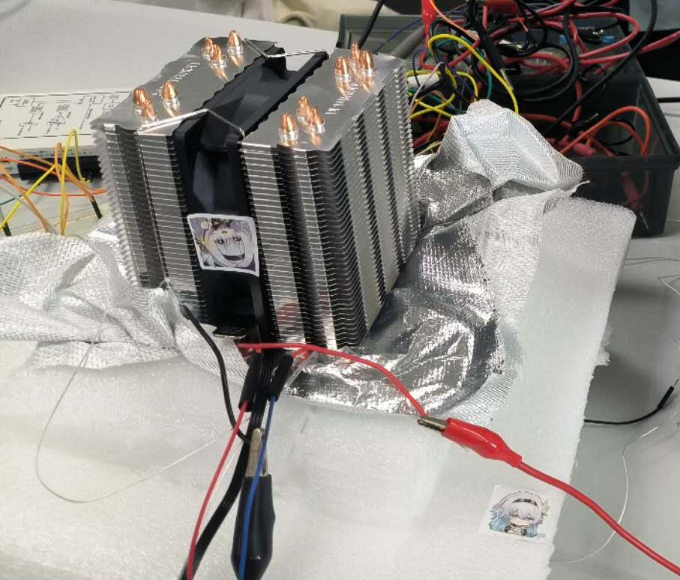
\includegraphics[width=0.45\textwidth]{热机实物图.png}\label{fig:热机实物图}}
        \hfill
        \subfloat[]{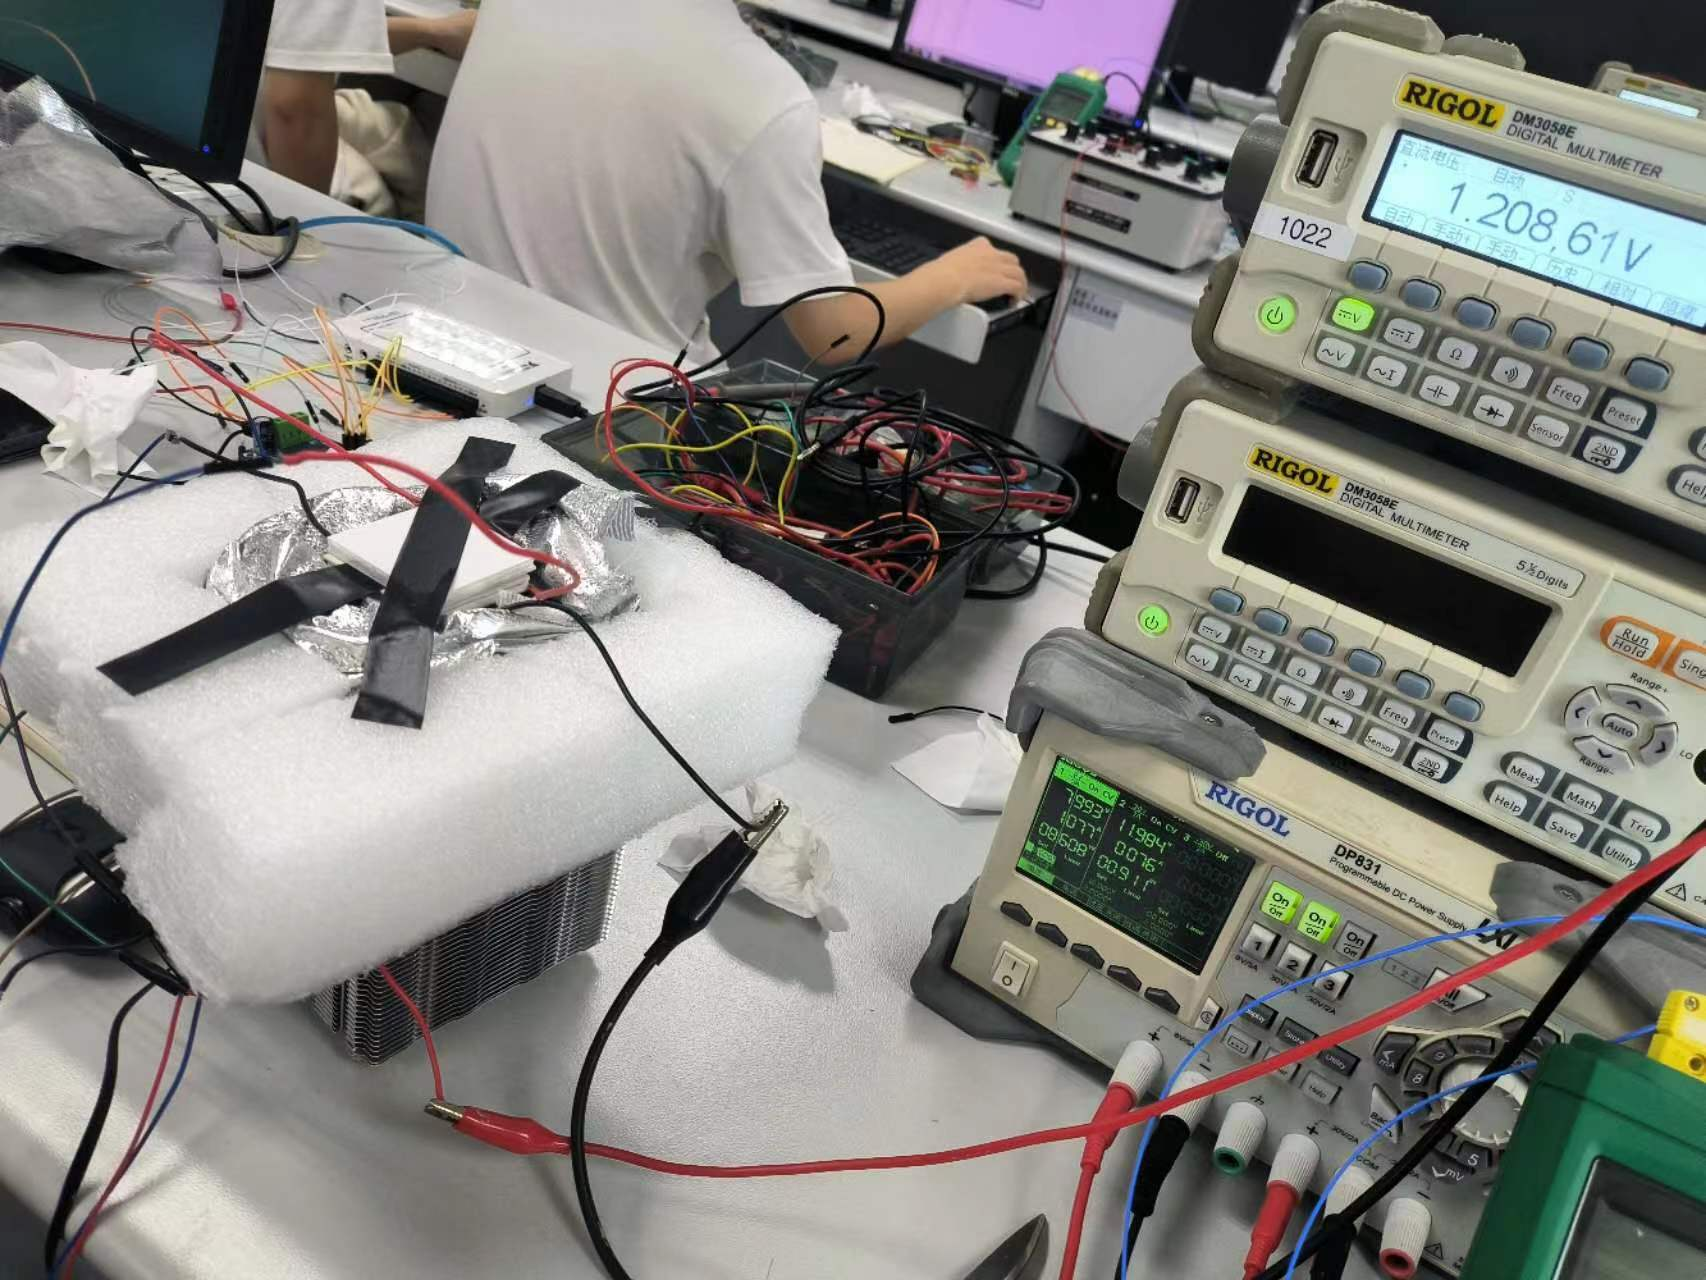
\includegraphics[width=0.45\textwidth]{热机实物图2.jpg}\label{fig:热机实物图2}}
        \hfill
        \subfloat[]{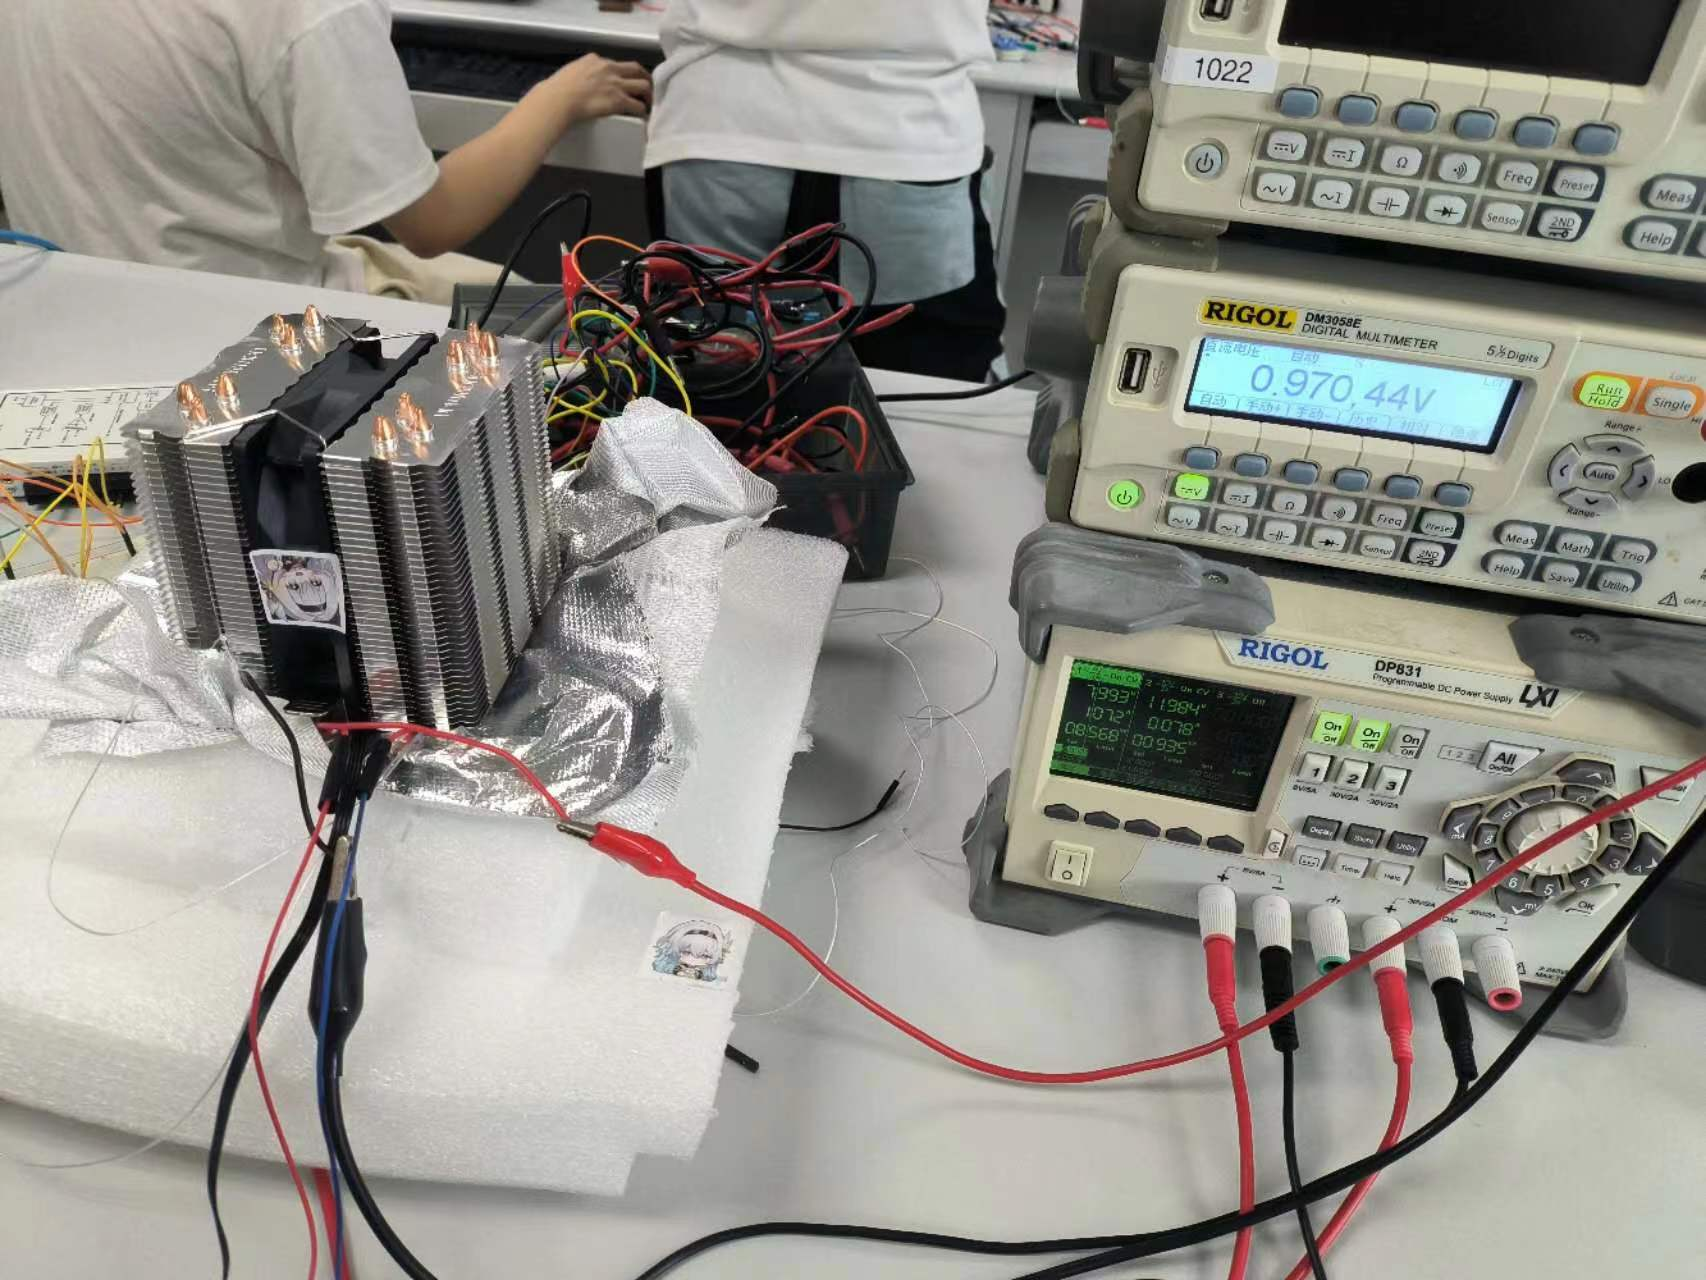
\includegraphics[width=0.45\textwidth]{热机实物图3.jpg}\label{fig:热机实物图3}}
        \caption{}
        \label{fig:热机}
    \end{figure}







\clearpage
\section{数据分析、误差讨论}

    \subsection{实验一 \ 测量热机外负载特性}

        首先,在固定冷热端温度的情况下,测量热机的外负载特性。热端使用电阻丝加热,使其固定功率工作,达到平衡后测量其温度为47℃;冷端取室温,即31℃。
        
        电路图如\cref{fig:电路图}所示。所接的外负载是一个滑动变阻器。由电路方程
        \[
            U_L = E - I \cdot R_L
        \]
        可知,只需改变电路的外负载,即可得到$U_L - I$的关系。所测数据如\cref{tbl:热机外负载特性测量数据}所示。电阻$R_L$由$R_L = \frac{U_L}{I}$得到,功率$P$由$P = U_L \cdot I$得到。使用方程$ U_L = E - I \cdot R_L $对数据进行线性拟合,得到\cref{fig:实验一1},即,热机的电动势$E = 1.08935 V$,内阻$R_s = 6.12 \Omega $。

        再使用公式$ P = (\frac{E}{R_L + R_s})^2 R_L $对数据中的$P$和$R_L$进行拟合,得到\cref{fig:实验一2},即热机电动势$E = 1.0856 V $,内阻$R_s = 6.069 \Omega $
        最大输出功率$P_{max} = 0.0485W $。




        \begin{figure}[htbp]
            \centering
            \subfloat[实验数据连线图1]{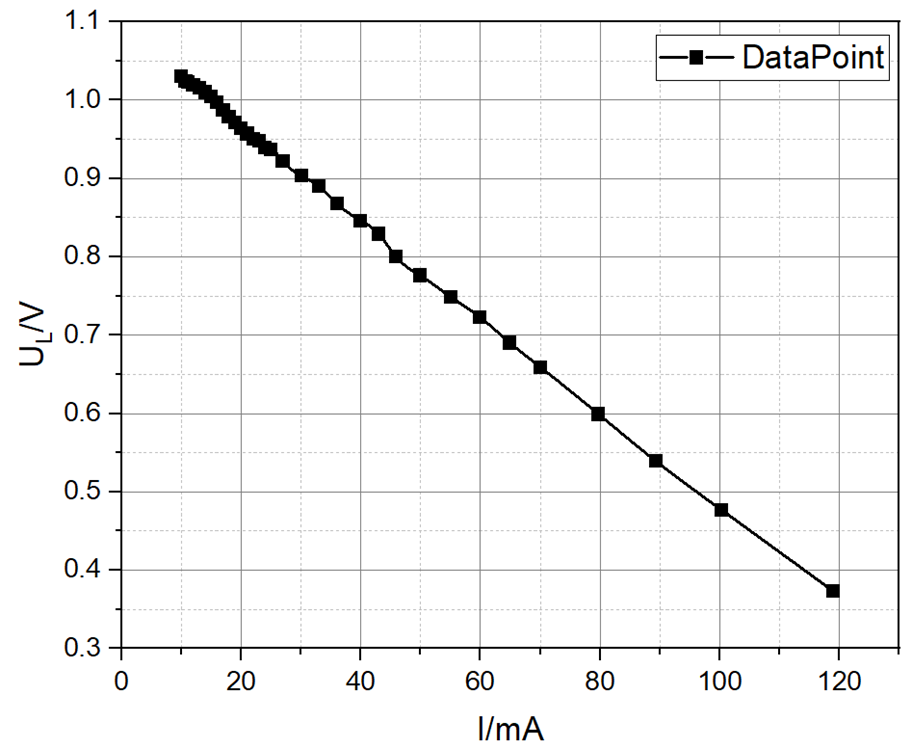
\includegraphics[width=0.47\textwidth]{实验一连线图1.png}\label{fig:实验一连线图1}}
            \hfill
            \subfloat[实验数据拟合图1]{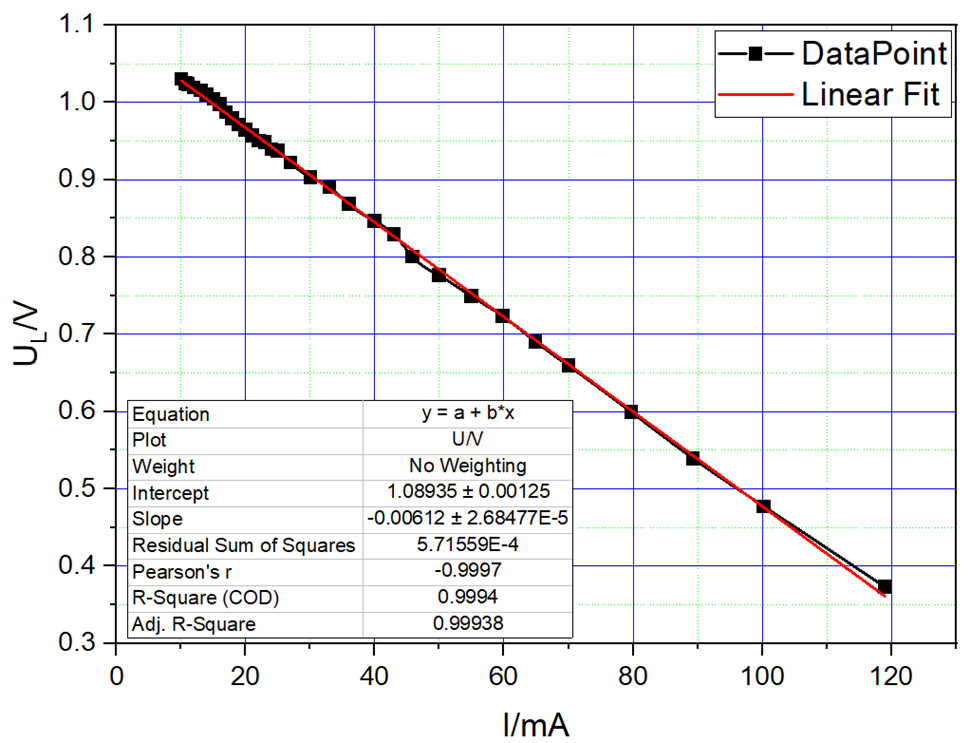
\includegraphics[width=0.5\textwidth]{实验一拟合图1.png}\label{fig:实验一拟合图1}}
            \caption{实验数据作图1}
            \label{fig:实验一1}
        \end{figure}

        \begin{figure}[htbp]
            \centering
            \subfloat[实验数据连线图2]{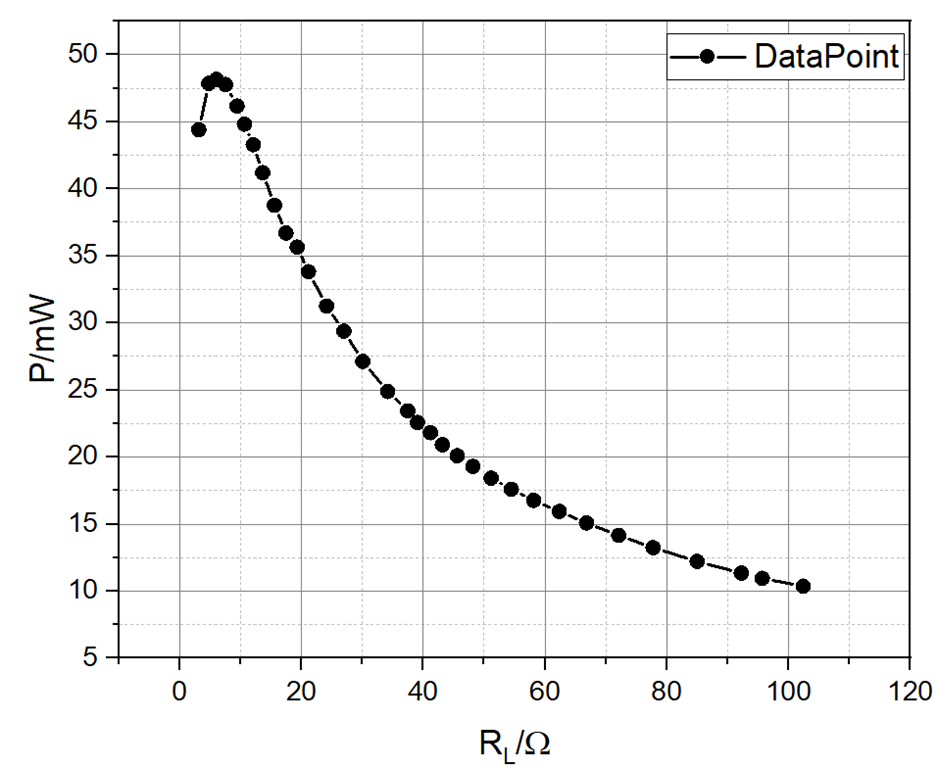
\includegraphics[width=0.5\textwidth]{实验一连线图2.png}\label{fig:实验一连线图2}}
            \hfill
            \subfloat[实验数据拟合图2]{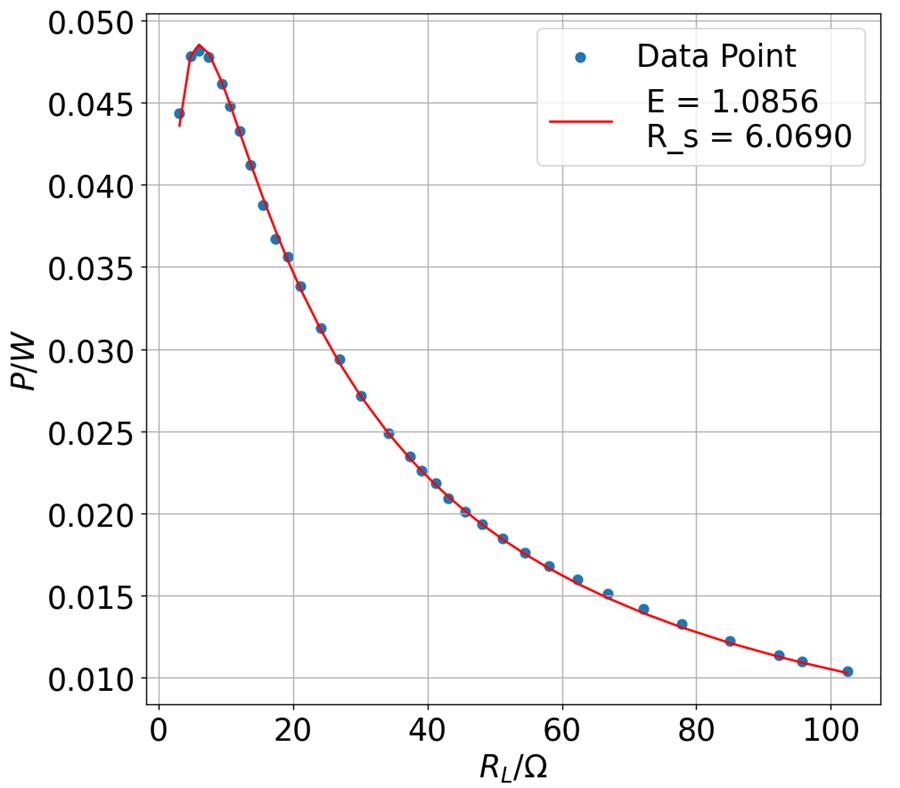
\includegraphics[width=0.47\textwidth]{实验一拟合图2.png}\label{fig:实验一拟合图2}}
            \caption{实验数据作图2}
            \label{fig:实验一2}
        \end{figure}


        \begin{table}
            \centering
            \begin{tblr}{
              vline{1,3,5,7,9} = {-}{},
              hline{1-2,19} = {-}{},
            }
            $U/V$   & $I/mA$   & $P/mW$   & $R_L/\Omega$  & $U/V$   & $I/mA$    & $P/mW$   & $R_L/\Omega$ \\
            1.030 & 10.055 & 10.357 & 102.437 & 0.937 & 25.020  & 23.444 & 37.450 \\
            1.024 & 10.700 & 10.957 & 95.701  & 0.922 & 26.980  & 24.876 & 34.173 \\
            1.023 & 11.090 & 11.345 & 92.245  & 0.903 & 30.040  & 27.126 & 30.060 \\
            1.019 & 11.990 & 12.218 & 84.987  & 0.890 & 33.010  & 29.379 & 26.962 \\
            1.015 & 13.050 & 13.246 & 77.778  & 0.868 & 36.010  & 31.257 & 24.104 \\
            1.010 & 14.007 & 14.147 & 72.107  & 0.846 & 39.980  & 33.823 & 21.161 \\
            1.004 & 15.025 & 15.085 & 66.822  & 0.829 & 43.000  & 35.647 & 19.279 \\
            0.997 & 15.990 & 15.942 & 62.351  & 0.800 & 45.860  & 36.688 & 17.444 \\
            0.987 & 16.980 & 16.759 & 58.127  & 0.776 & 49.950  & 38.761 & 15.536 \\
            0.979 & 17.970 & 17.593 & 54.480  & 0.749 & 55.010  & 41.202 & 13.616 \\
            0.971 & 18.980 & 18.430 & 51.159  & 0.723 & 59.860  & 43.279 & 12.078 \\
            0.964 & 20.020 & 19.299 & 48.152  & 0.690 & 64.950  & 44.816 & 10.624 \\
            0.957 & 21.000 & 20.097 & 45.571  & 0.659 & 70.050  & 46.163 & 9.408  \\
            0.950 & 22.020 & 20.919 & 43.143  & 0.599 & 79.750  & 47.770 & 7.511  \\
            0.948 & 23.010 & 21.813 & 41.199  & 0.539 & 89.350  & 48.160 & 6.032  \\
            0.939 & 24.040 & 22.574 & 39.060  & 0.477 & 100.300 & 47.843 & 4.756  \\
                  &        &        &         & 0.373 & 119.020 & 44.394 & 3.134  
            \end{tblr}
            \caption{热机外负载特性测量数据}
            \label{tbl:热机外负载特性测量数据}
        \end{table}



        \textbf{不确定度评定:}
        
            
            假设电压 \( U \) 和电流 \( I \) 的测量误差分别是±0.1\%的测量值加上一个固定的仪器误差,这里我们假设为±0.005 V和±0.1 mA。图像如\cref{fig:实验一误差棒图}

            \begin{enumerate}
                 \item 电压 U 的不确定度 \( u(U) \):
                        
                    \[ u(U) = \sqrt{ ( 0.1\% U)^2 + (0.005 \text{ V})^2} \]
                    
                    \item 电流 I 的不确定度 \( u(I) \):
                    
                    \[ u(I) = \sqrt{ ( 0.1\% I)^2 + (0.1 \text{ mA})^2} \]
                    
            \end{enumerate}

            同理可得,$P=UI$与$R_L=\frac{U}{I}$的不确定度,如\cref{tbl:热机外负载特性的误差评定}所示,作图如\cref{fig:实验数据作图+误差棒1}。
                

                % 数据的不确定度计算
                
                % 下面,我会根据这些公式和你提供的数据来计算每一行数据的不确定度。
                
                % 示例计算
                
                % 以第一行数据为例:
                % - \( U = 1.030 \) V, \( I = 10.055 \) mA
                % - \( u(U) = \sqrt{(0.00103)^2 + (0.005)^2} \)
                % - \( u(I) = \sqrt{(0.010055)^2 + (0.1)^2} \)

                \begin{figure}[htbp]
                    \centering
                    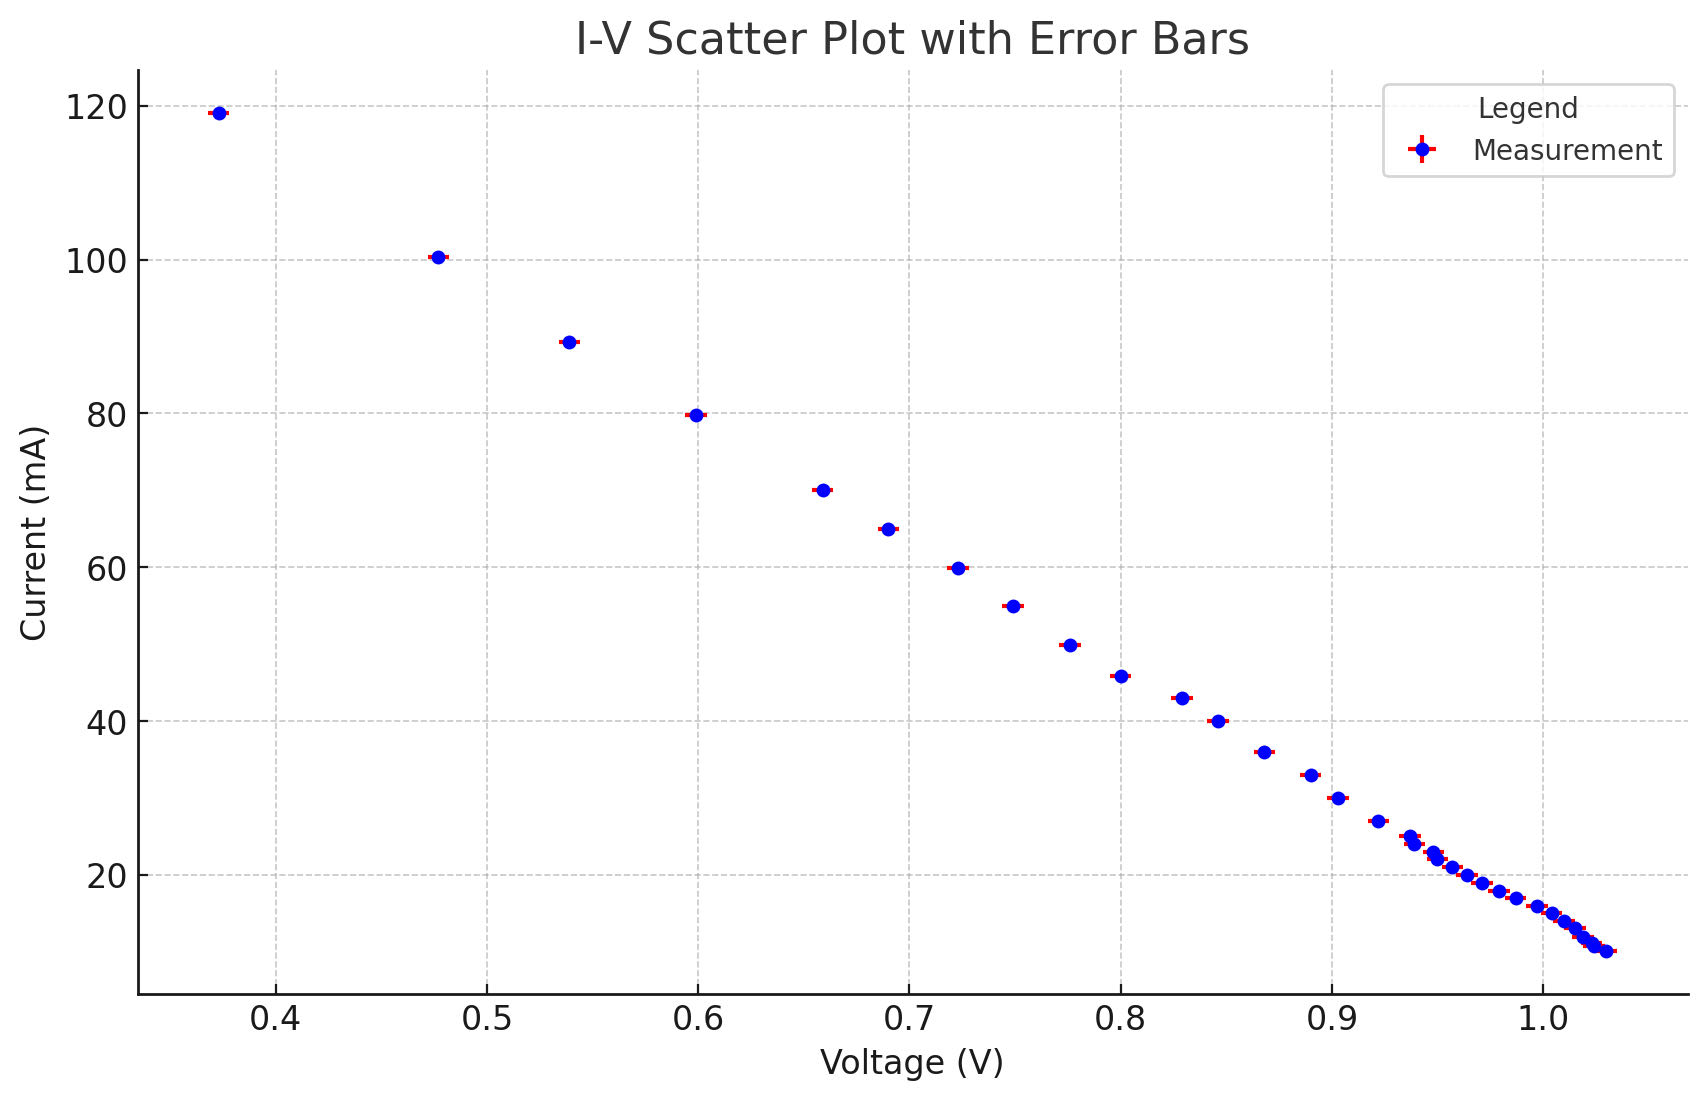
\includegraphics[width=0.8\textwidth]{实验一误差棒图.jpg}
                    \caption{热机外负载特性测量+误差棒}
                    \label{fig:实验一误差棒图}
                \end{figure}


                \begin{figure}[htbp]
                    \centering
                    % \subfloat[热机外负载特性测量电压、电流+误差棒]{\includegraphics[width=0.5\textwidth]{U-I图+误差棒.jpg}\label{fig:U-I图+误差棒}}
                    % \hfill
                    \subfloat[热机外负载特性测量输出功率、负载电阻+误差棒]{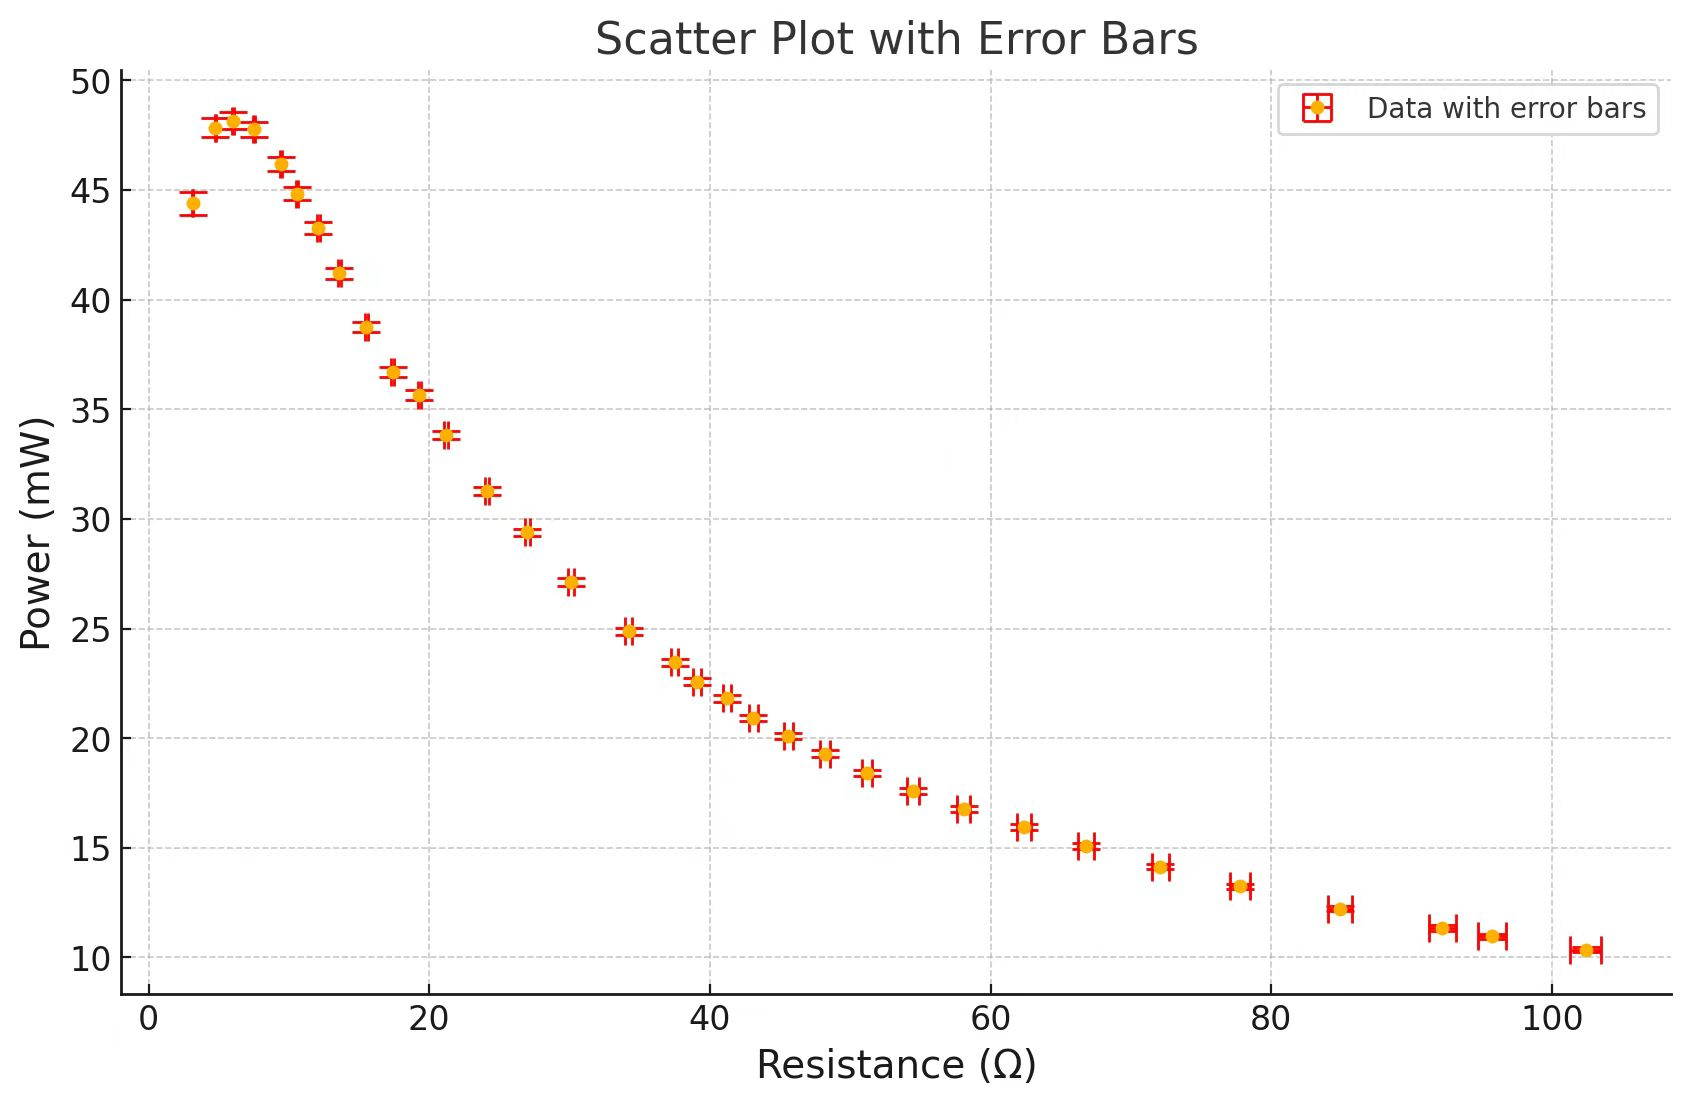
\includegraphics[width=0.47\textwidth]{P-R图+误差棒.jpg}\label{fig:P-R图+误差棒}}
                    \caption{实验数据作图+误差棒}
                    \label{fig:实验数据作图+误差棒1}
                \end{figure}

                \begin{longtable}{|c|c|c|c|c|c|c|c|}
                    \caption{热机外负载特性的误差评定}
                    \label{tbl:热机外负载特性的误差评定} \\
                    \hline
                    $U/V$ & $I/mA$ & $u(U)/V$ & $u(I)/mA$ & $P/mW$ & $u(P)/mW$ & $R/\Omega$ & $u(R)/\Omega$ \\
                    \hline
                    \endfirsthead
                    \caption[]{热机外负载特性的误差评定 (续)} \\
                    \hline
                    $U/V$ & $I/mA$ & $u(U)/V$ & $u(I)/mA$ & $P/mW$ & $u(P)/mW$ & $R/\Omega$ & $u(R)/\Omega$ \\
                    \hline
                    \endhead
                    \hline
                    \endfoot
                    
                    \hline
                    1.03  & 10.055 & 0.0051 & 0.1005 & 10.357 & 0.116 & 102.4 & 1.1 \\
                    1.024 & 10.7 & 0.0051 & 0.1006 & 10.957 & 0.117 & 95.7 & 1 \\
                    1.023 & 11.09 & 0.0051 & 0.1006 & 11.345 & 0.117 & 92.2 & 0.96 \\
                    1.019 & 11.99 & 0.0051 & 0.1007 & 12.218 & 0.119 & 84.9 & 0.83 \\
                    1.015 & 13.05 & 0.0051 & 0.1008 & 13.246 & 0.122 & 77.8 & 0.72 \\
                    1.01  & 14.007 & 0.0051 & 0.1009 & 14.147 & 0.125 & 72.1 & 0.63 \\
                    1.004 & 15.025 & 0.0051 & 0.1012 & 15.085 & 0.127 & 66.8 & 0.56 \\
                    0.997 & 15.99 & 0.0051 & 0.1013 & 15.942 & 0.13 & 62.4 & 0.51 \\
                    0.987 & 16.98 & 0.0051 & 0.1014 & 16.759 & 0.132 & 58.1 & 0.46 \\
                    0.979 & 17.97 & 0.0051 & 0.1017 & 17.593 & 0.135 & 54.5 & 0.42 \\
                    0.971 & 18.98 & 0.0051 & 0.1017 & 18.43 & 0.138 & 51.2 & 0.38 \\
                    0.964 & 20.02 & 0.0051 & 0.102 & 19.299 & 0.142 & 48.2 & 0.35 \\
                    0.957 & 21.00 & 0.0051 & 0.1022 & 20.097 & 0.145 & 45.6 & 0.33 \\
                    0.95  & 22.02 & 0.0051 & 0.1024 & 20.919 & 0.148 & 43.1 & 0.31 \\
                    0.948 & 23.01 & 0.0051 & 0.1026 & 21.811 & 0.151 & 41.2 & 0.29 \\
                    0.939 & 24.04 & 0.0051 & 0.1028 & 22.578 & 0.154 & 39.1 & 0.27 \\
                    0.937 & 25.02 & 0.0051 & 0.1031 & 23.454 & 0.157 & 37.5 & 0.26 \\
                    0.922 & 26.98 & 0.0051 & 0.1036 & 24.868 & 0.162 & 34.2 & 0.23 \\
                    0.903 & 30.04 & 0.0051 & 0.1044 & 27.126 & 0.17 & 30.1 & 0.2 \\
                    0.89  & 33.01 & 0.0051 & 0.1053 & 29.379 & 0.179 & 27 & 0.18 \\
                    0.868 & 36.01 & 0.0051 & 0.1063 & 31.257 & 0.189 & 24.1 & 0.16 \\
                    0.846 & 39.98 & 0.0051 & 0.1077 & 33.823 & 0.202 & 21.2 & 0.14 \\
                    0.829 & 43 & 0.0051 & 0.1089 & 35.647 & 0.214 & 19.3 & 0.13 \\
                    0.8   & 45.86 & 0.0051 & 0.11 & 36.688 & 0.224 & 17.4 & 0.12 \\
                    0.776 & 49.95 & 0.0051 & 0.1118 & 38.761 & 0.238 & 15.5 & 0.11 \\
                    0.749 & 55.01 & 0.0051 & 0.1141 & 41.202 & 0.258 & 13.6 & 0.096 \\
                    0.723 & 59.86 & 0.0051 & 0.1165 & 43.279 & 0.277 & 12.1 & 0.088 \\
                    0.69  & 64.95 & 0.005 & 0.1192 & 44.816 & 0.296 & 10.6 & 0.08 \\
                    0.659 & 70.05 & 0.005 & 0.122 & 46.163 & 0.317 & 9.41 & 0.074 \\
                    0.599 & 79.75 & 0.005 & 0.1279 & 47.77 & 0.349 & 7.51 & 0.064 \\
                    0.539 & 89.35 & 0.005 & 0.1341 & 48.16 & 0.387 & 6.03 & 0.057 \\
                    0.477 & 100.3 & 0.005 & 0.1416 & 47.843 & 0.431 & 4.76 & 0.05 \\
                    0.373 & 119.02 & 0.005 & 0.1555 & 44.394 & 0.516 & 3.13 & 0.042 \\
                \end{longtable}



    \subsection{Seebeck系数测量}

        \begin{table}[htbp]
            \centering
            % \small
            \resizebox{\textwidth}{!}{%
                \begin{tabular}{|c|cccccccccccccccc|} 
                \hline
                温差
                (°C) & 10    & 11    & 12    & 13    & 14    & 15    & 16   & 17    & 18    & 19    & 20    & 21    & 22    & 23    & 24    & 25     \\
                开路电压 (V)  & 0.602 & 0.689 & 0.736 & 0.798 & 0.928 & 0.951 & 1.05 & 1.065 & 1.156 & 1.267 & 1.284 & 1.426 & 1.472 & 1.546 & 1.617 & 1.837  \\
                \hline
                \end{tabular}
            }
            \caption{Seebeck系数测量数据}
            \label{tbl:Seebeck系数测量数据}
        \end{table}

        在Seebeck系数测量实验中,我们使风扇全功率运行,并让热端缓慢升温,可以认为冷端温度为定值,即室温31℃;在热端缓慢升温的过程中,每隔1℃读出其开路电压,测量数据如\cref{tbl:Seebeck系数测量数据}所示。

        对该组数据进行线性拟合,得到图像如\cref{fig:实验二拟合图1},即Seebeck系数$\alpha = 0.0756 V/K$


        
        \begin{figure}[htbp]
            \centering
            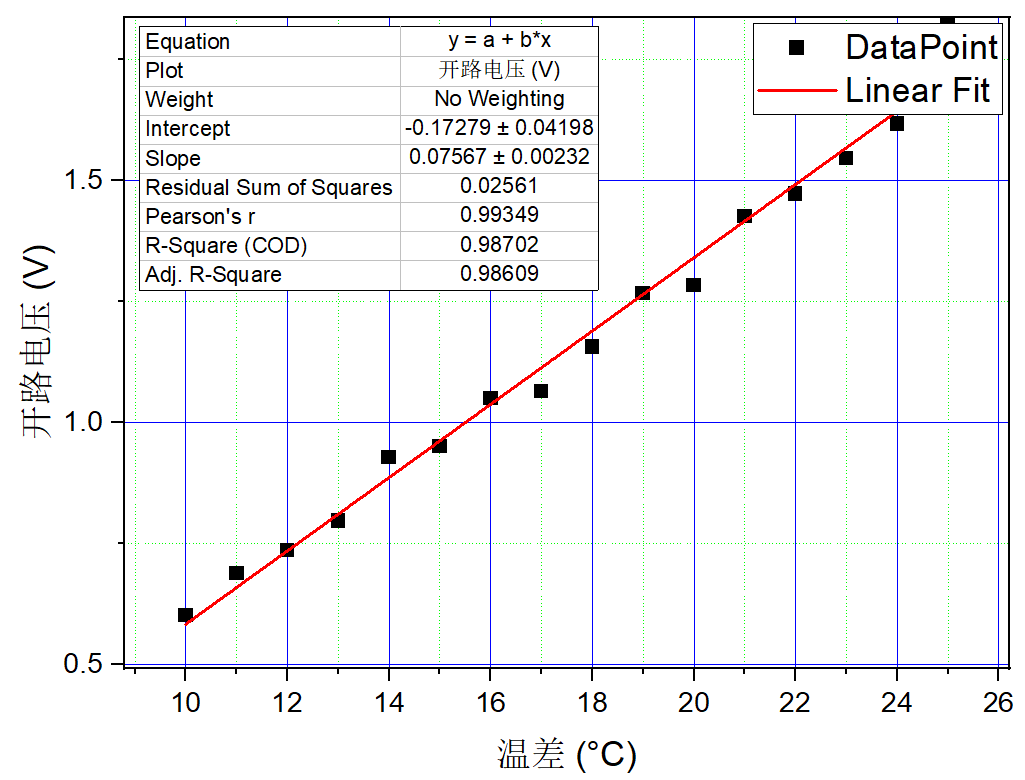
\includegraphics[width=0.6\textwidth]{实验二拟合图1.png}
            \caption{Seebeck系数测量拟合}
            \label{fig:实验二拟合图1}
        \end{figure}

        下面是不确定度分析:

        Seebeck系数 \(S\) 可以通过温差 (\( \Delta T \)) 和相应的开路电压 (\( V \)) 计算得出:
        \[ S = \frac{V}{\Delta T} \]
        对于给定的数据,Seebeck系数的计算结果如下:
        \begin{align*}
        S_{10} &= \frac{0.602}{10} = 0.0602, \\
        S_{11} &= \frac{0.689}{11} = 0.0626, \\
        &\vdots \\
        S_{25} &= \frac{1.837}{25} = 0.0735.
        \end{align*}

        \[ u_A = \frac{\sigma_S}{\sqrt{n}} \]
        其中,\( \sigma_S \) 是Seebeck系数样本的标准偏差,\( n \) 是样本数量。

        计算得到的A类不确定度为:
        \[ u_A = \frac{0.00503}{\sqrt{16}} = 0.000826 \]

        \[ u_B = S \sqrt{\left(\frac{\delta V}{V}\right)^2 + \left(\frac{\delta T}{T}\right)^2} \]
        其中,\( \delta V \) 和 \( \delta T \) 分别是电压和温度的测量精度。

        对于每一组数据的B类不确定度平均值为:
        \[ \text{平均 } u_B = 0.000402 \]

        合并不确定度是将A类和B类不确定度合并:
        \[ u_C = \sqrt{u_A^2 + u_B^2} \]
        计算得到的合并不确定度为:
        \[ u_C = \sqrt{0.000826^2 + 0.000402^2} = 0.000919 \]

        采用95\%置信度(约为2倍标准偏差)计算展伸不确定度:
        \[ U = k \times u_C \]
        其中,\( k \) 是覆盖因子,通常为2。
        \[ U = 2 \times 0.000919 = 0.001837 \]










    \subsection{TEC内阻与输出功率分析}

        \textbf{不确定度评定:}

        设我们测得的电压 \( U \) 和电流 \( I \) 的不确定度分别为:$\sigma_U$和$\sigma_I$

        
        由公式 \( U = E - rI \),其中 \( E \) 是电动势,\( r \) 是内阻,通过测量 \( I \) 和 \( U \) 并线性拟合,可得到内阻 \( r \) 的值及其不确定度。公式为:
        
        \[ r = \frac{\Delta U}{\Delta I} \]
        
        根据误差传递公式,内阻的不确定度 \( \sigma_r \) 为:
        
        \[ \sigma_r = \sqrt{\left( \frac{\partial r}{\partial U} \sigma_U \right)^2 + \left( \frac{\partial r}{\partial I} \sigma_I \right)^2} = \sqrt{\left( \frac{1}{\Delta I} \sigma_U \right)^2 + \left( \frac{\Delta U}{(\Delta I)^2} \sigma_I \right)^2} \]
        

        
        通过以上方法,利用不同温差下的 \( \Delta U \) 和 \( \Delta I \) 来计算各温差下内阻及其不确定度,然后利用 95\% 置信区间的展伸因子 (k=2) 计算展伸不确定度$ U_r = k \cdot \sigma_r $。最后处理的数据见\cref{tbl:TEC内阻随温差变化数据},作图见\cref{fig:TEC内阻随温差变化分析+误差棒}。

        同时绘制输出功率与温差的关系图,见\cref{fig:输出功率--温差}。由公式$P_{\text{out}} = \frac{(\alpha \Delta T)^2 \cdot R_{\text{L}}}{(R_{\text{L}} + R_{\text{s}})^2}$可知,$P_{out} \propto (\Delta T)^2 $,但是图中的二次关系并不明显,可能的原因是内阻值也在随温差的变化而变化。
        
        % \[ U_r = k \times \sigma_r \]




        \begin{table}[htbp]
            \centering
            \begin{tabular}{|cc|cc|} 
            \hline
            $\Delta T/K$ & $R_s/\Omega$ & $u(R_s)/\Omega$ & $u_{extended}(R_s)$  \\ 
            \hline
            10   & 2.947       & 0.185   & 0.370      \\
            11   & 3.582       & 0.180   & 0.360      \\
            12   & 3.555       & 0.172   & 0.344      \\
            13   & 5.134       & 0.190   & 0.380      \\
            14   & 5.059       & 0.178   & 0.356      \\
            15   & 4.786       & 0.181   & 0.362      \\
            16   & 6.332       & 0.176   & 0.352      \\
            17   & 5.766       & 0.189   & 0.378      \\
            18   & 5.356       & 0.174   & 0.348      \\
            19   & 6.141       & 0.192   & 0.384      \\
            20   & 5.619       & 0.177   & 0.354      \\
            21   & 5.551       & 0.184   & 0.368      \\
            22   & 4.153       & 0.179   & 0.358      \\
            23   & 5.231       & 0.182   & 0.364      \\
            24   & 4.486       & 0.175   & 0.350      \\
            25   & 2.713       & 0.186   & 0.372      \\
            \hline
            \end{tabular}
            \caption{TEC内阻随温差变化数据}
            \label{tbl:TEC内阻随温差变化数据}
        \end{table}

        \begin{figure}[htbp]
            \centering
            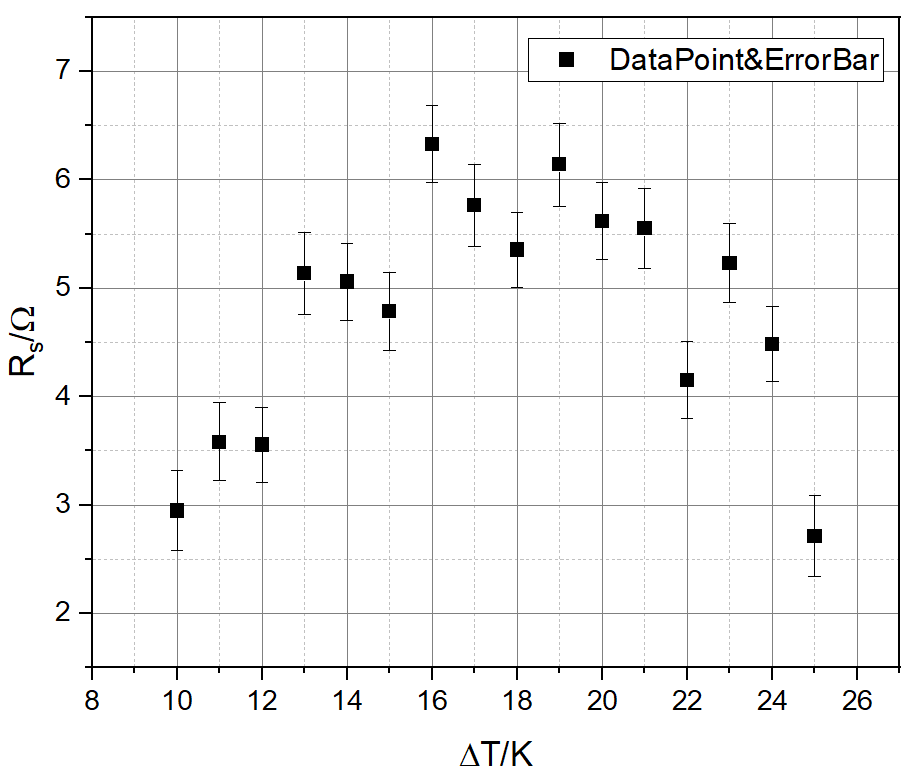
\includegraphics[width=0.6\textwidth]{TEC内阻--温差+误差棒.png}
            \caption{TEC内阻随温差变化分析+误差棒}
            \label{fig:TEC内阻随温差变化分析+误差棒}
        \end{figure}

        


        \begin{figure}[htbp]
            \centering
            \subfloat[输出功率--温差连线图]{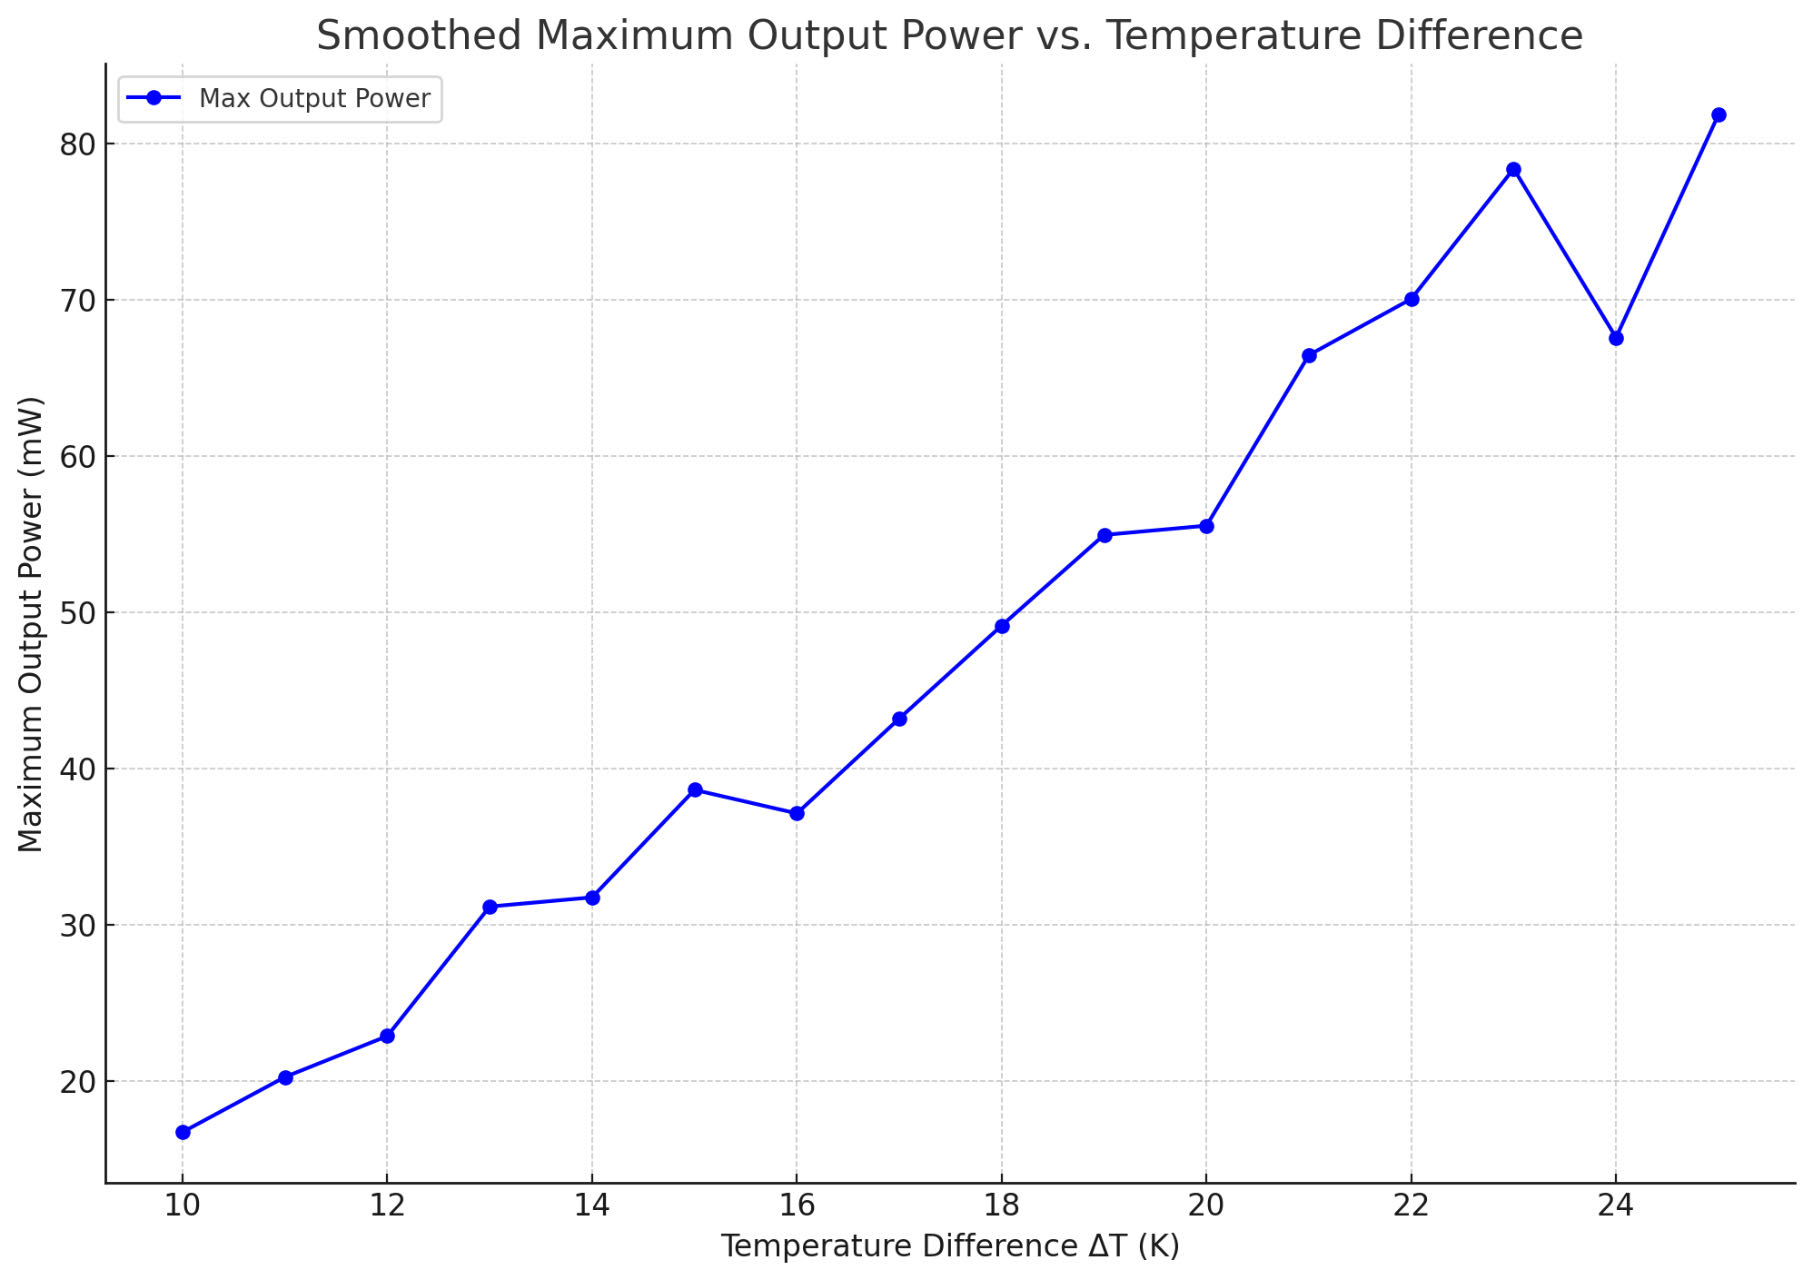
\includegraphics[width=0.5\textwidth]{输出功率--温差连线图.jpg}\label{fig:输出功率--温差连线图}}
            \hfill
            \subfloat[输出功率--温差误差棒]{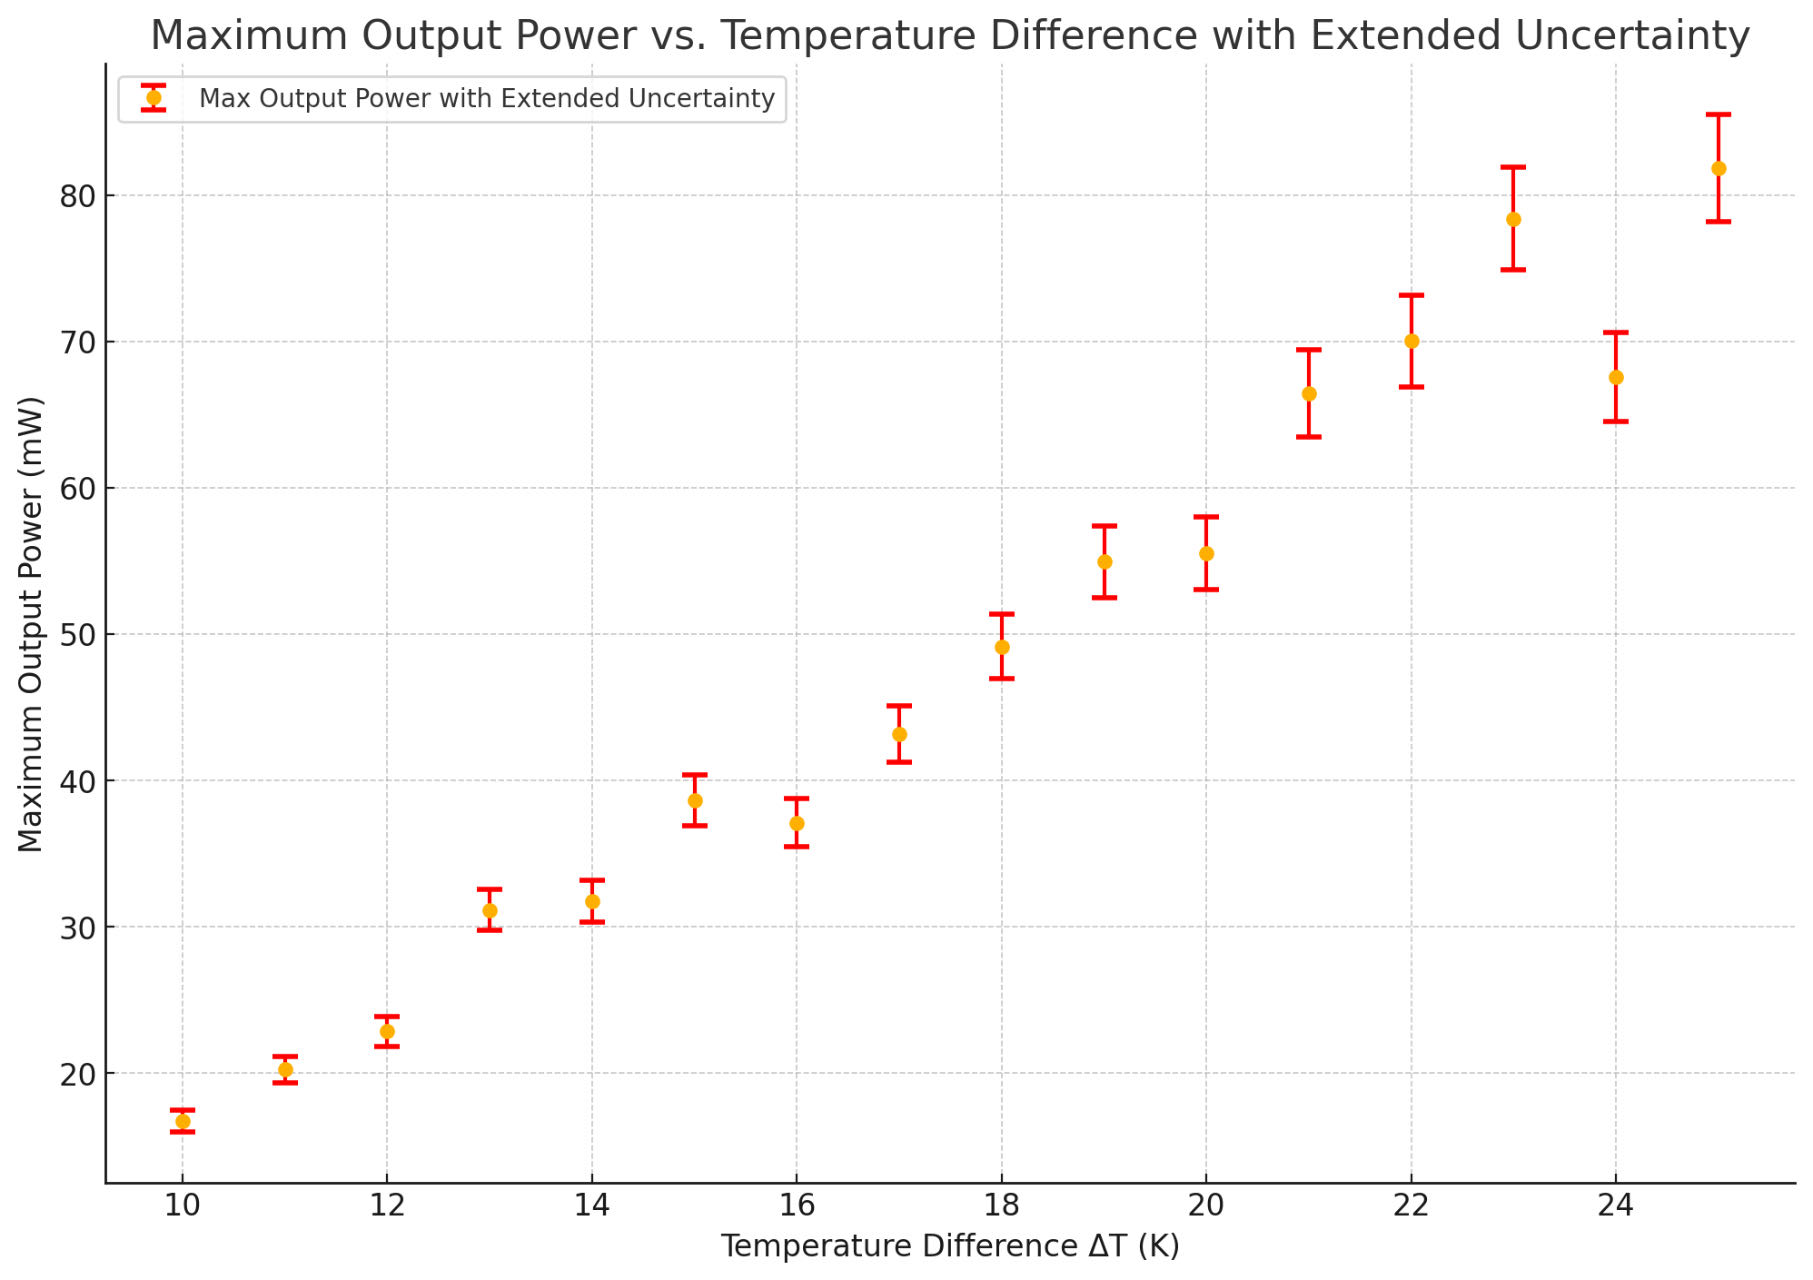
\includegraphics[width=0.47\textwidth]{输出功率--温差误差棒.jpg}\label{fig:输出功率--温差误差棒}}
            \caption{输出功率--温差误差棒}
            \label{fig:输出功率--温差}
        \end{figure}


    
\clearpage

    \subsection{双TEC耦合热电堆}

        \textbf{不确定度评定:}
        
        首先,计算电压 \( U \) 和电流 \( I \) 的B类不确定度。接着,使用这些不确定度来计算功率 \( P \) 和电阻 \( R \) 以及它们的不确定度。最后,计算展伸不确定度(扩展至95\%置信区间,通常使用k=2)。

        假设测量误差分布同前,电压 \( U \) 和电流 \( I \) 的测量误差分别为±0.1\%的测量值加上一个固定的仪器误差,设为±0.005 V和±0.1 mA。

        \[ P = U \times I \]
        \[ R = \frac{U}{I} \]

        \[ u(P) = \sqrt{(I \cdot u(U))^2 + (U \cdot u(I))^2} \]
        \[ u(R) = \sqrt{\left(\frac{u(U)}{I}\right)^2 + \left(\frac{U \cdot u(I)}{I^2}\right)^2} \]

        \[ u_{\text{expanded}}(P) = k \cdot u(P) \]
        \[ u_{\text{expanded}}(R) = k \cdot u(R) \]
        其中 \( k = 2 \)。

        \begin{enumerate}


            \item 并联电流耦合

                数据见\cref{tbl:串联的外输出特性},误差棒作图如\cref{fig:双TEC片并联电流耦合数据处理}


                \begin{figure}[htbp]
                    \centering
                    \subfloat[并联电流耦合U-I+误差棒]{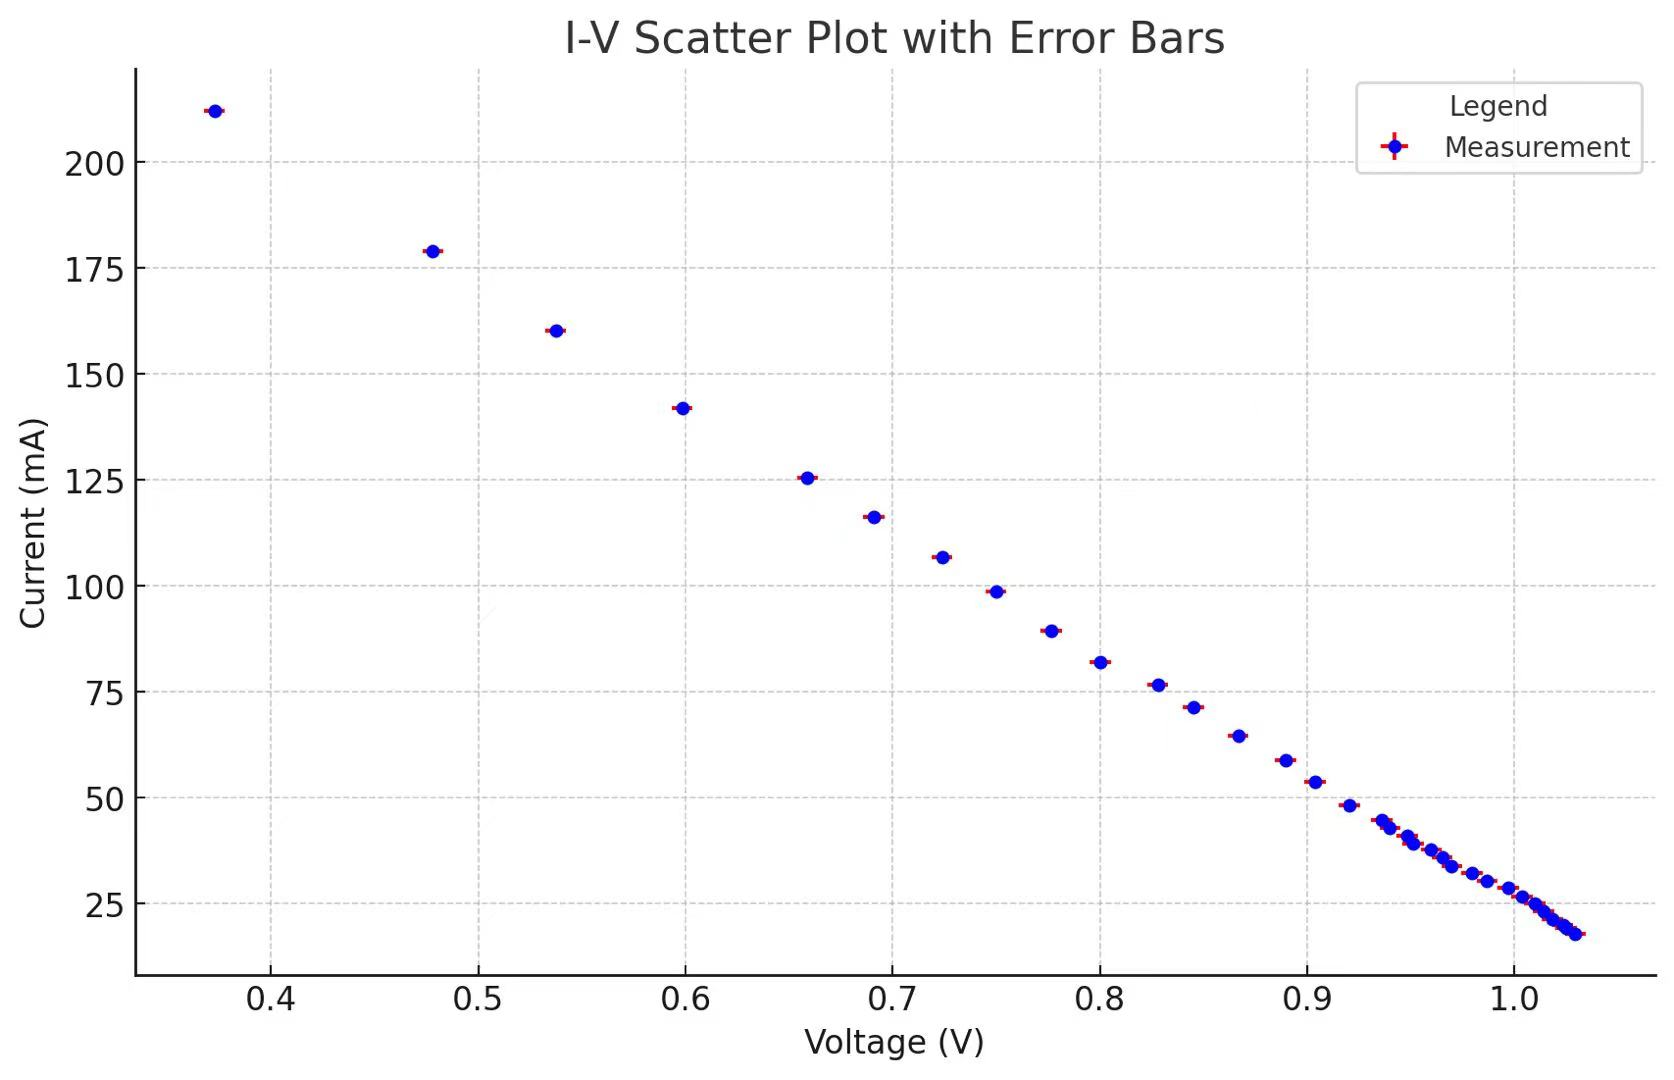
\includegraphics[width=0.5\textwidth]{并联电流耦合U-I+误差棒.jpg}\label{fig:并联电流耦合U-I+误差棒}}
                    \hfill
                    \subfloat[并联电流耦合P-R+误差棒]{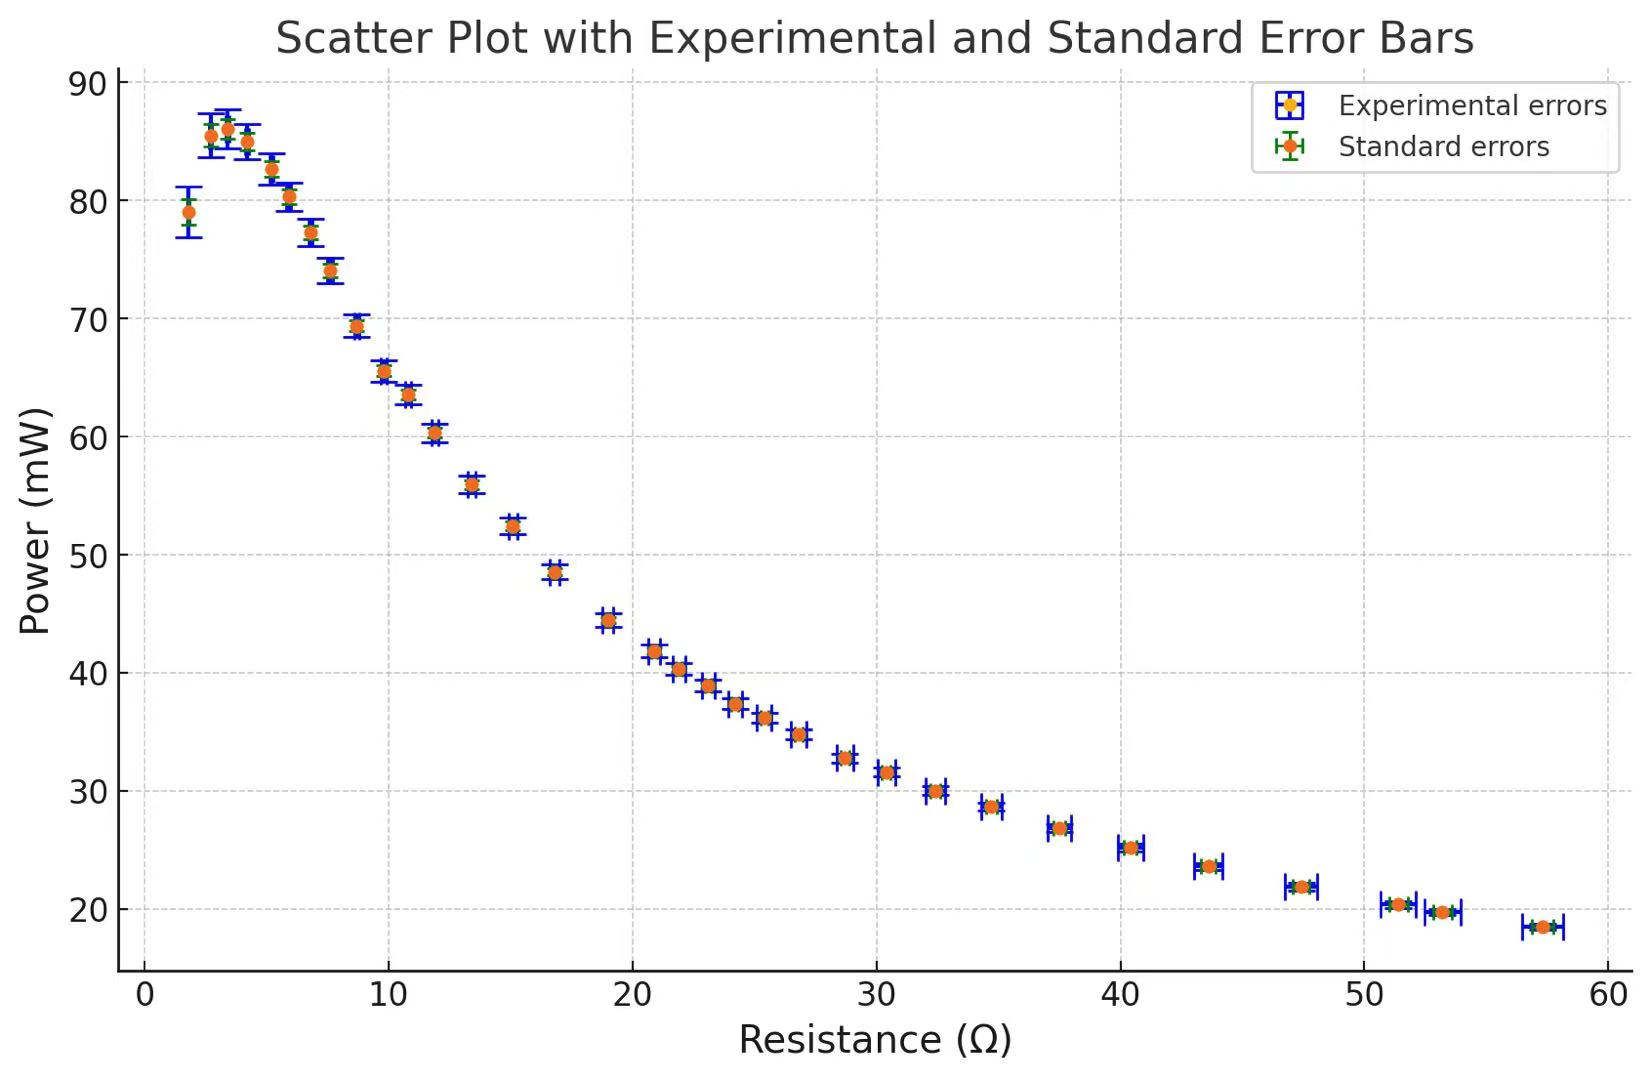
\includegraphics[width=0.47\textwidth]{并联电流耦合P-R+误差棒.jpg}\label{fig:并联电流耦合P-R+误差棒}}
                    \caption{双TEC片并联电流耦合数据处理+误差棒绘制}
                    \label{fig:双TEC片并联电流耦合数据处理}
                \end{figure}


            \item 并联电压耦合
            
                数据见\cref{tbl:并联的外输出特性},误差棒作图如\cref{fig:双TEC片并联电压耦合数据处理}

                
                \begin{figure}[htbp]
                    \centering
                    \subfloat[并联电压耦合U-I+误差棒]{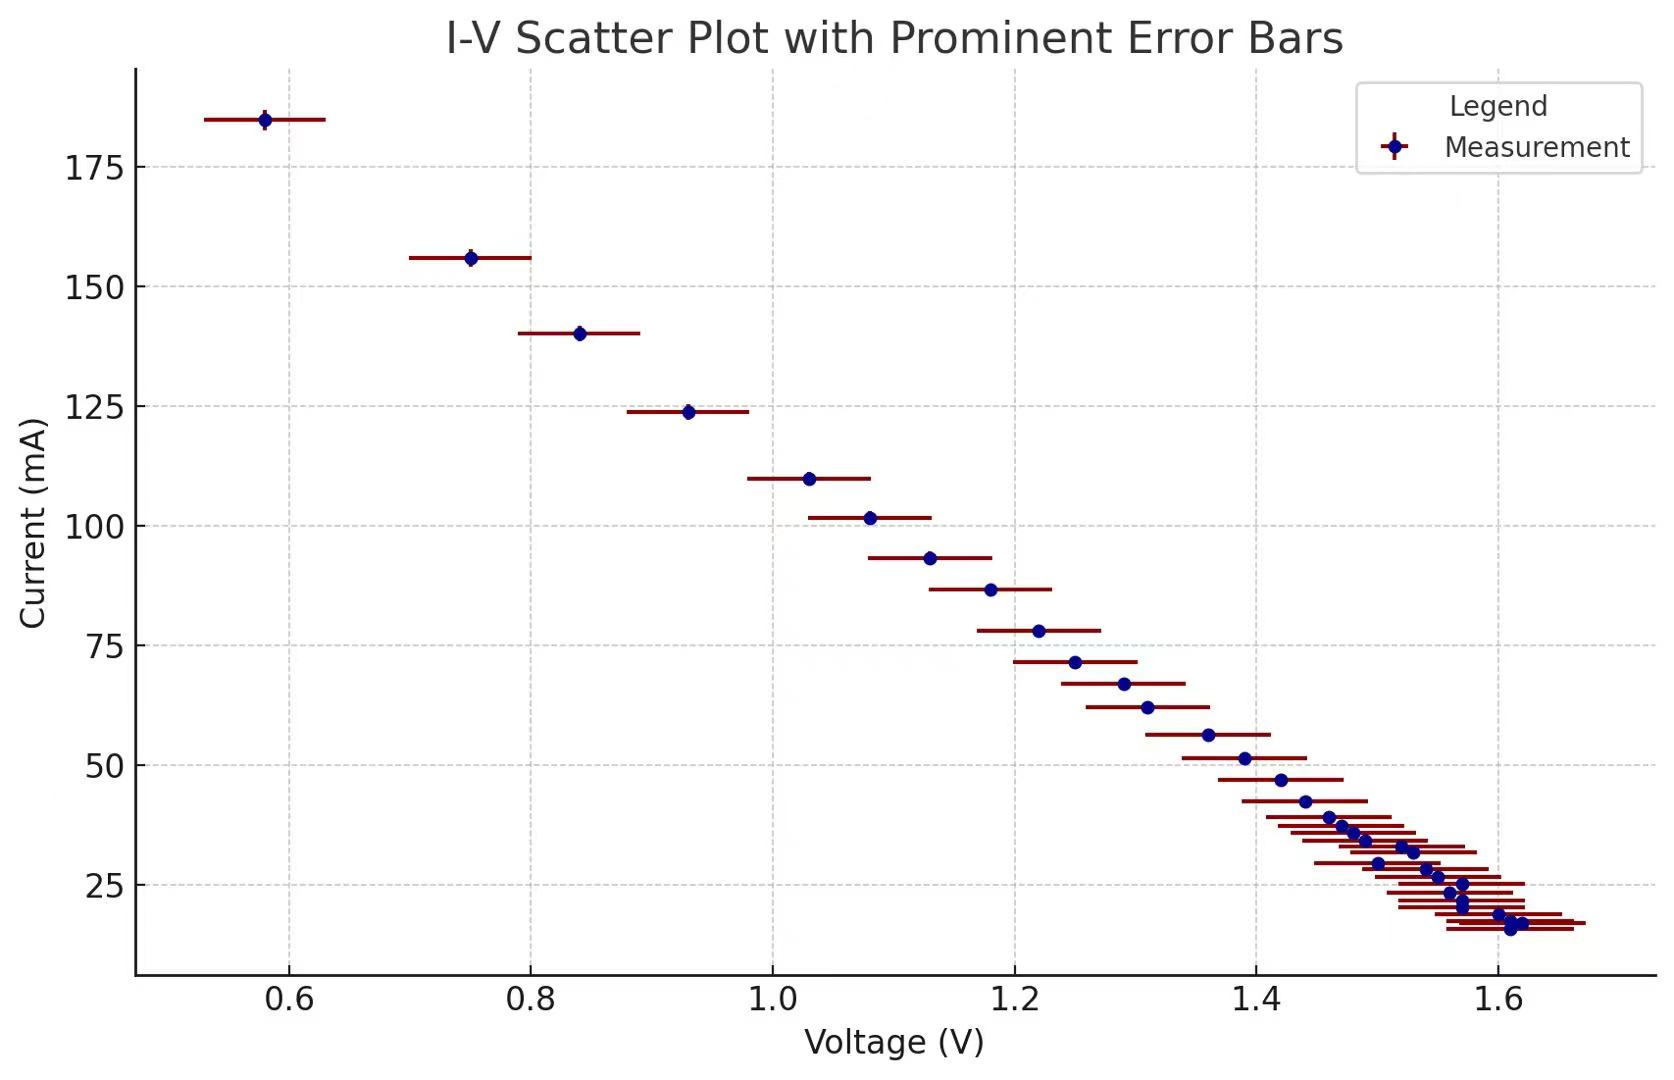
\includegraphics[width=0.5\textwidth]{并联电压耦合U-I+误差棒.jpg}\label{fig:并联电压耦合U-I+误差棒}}
                    \hfill
                    \subfloat[并联电压耦合P-R+误差棒]{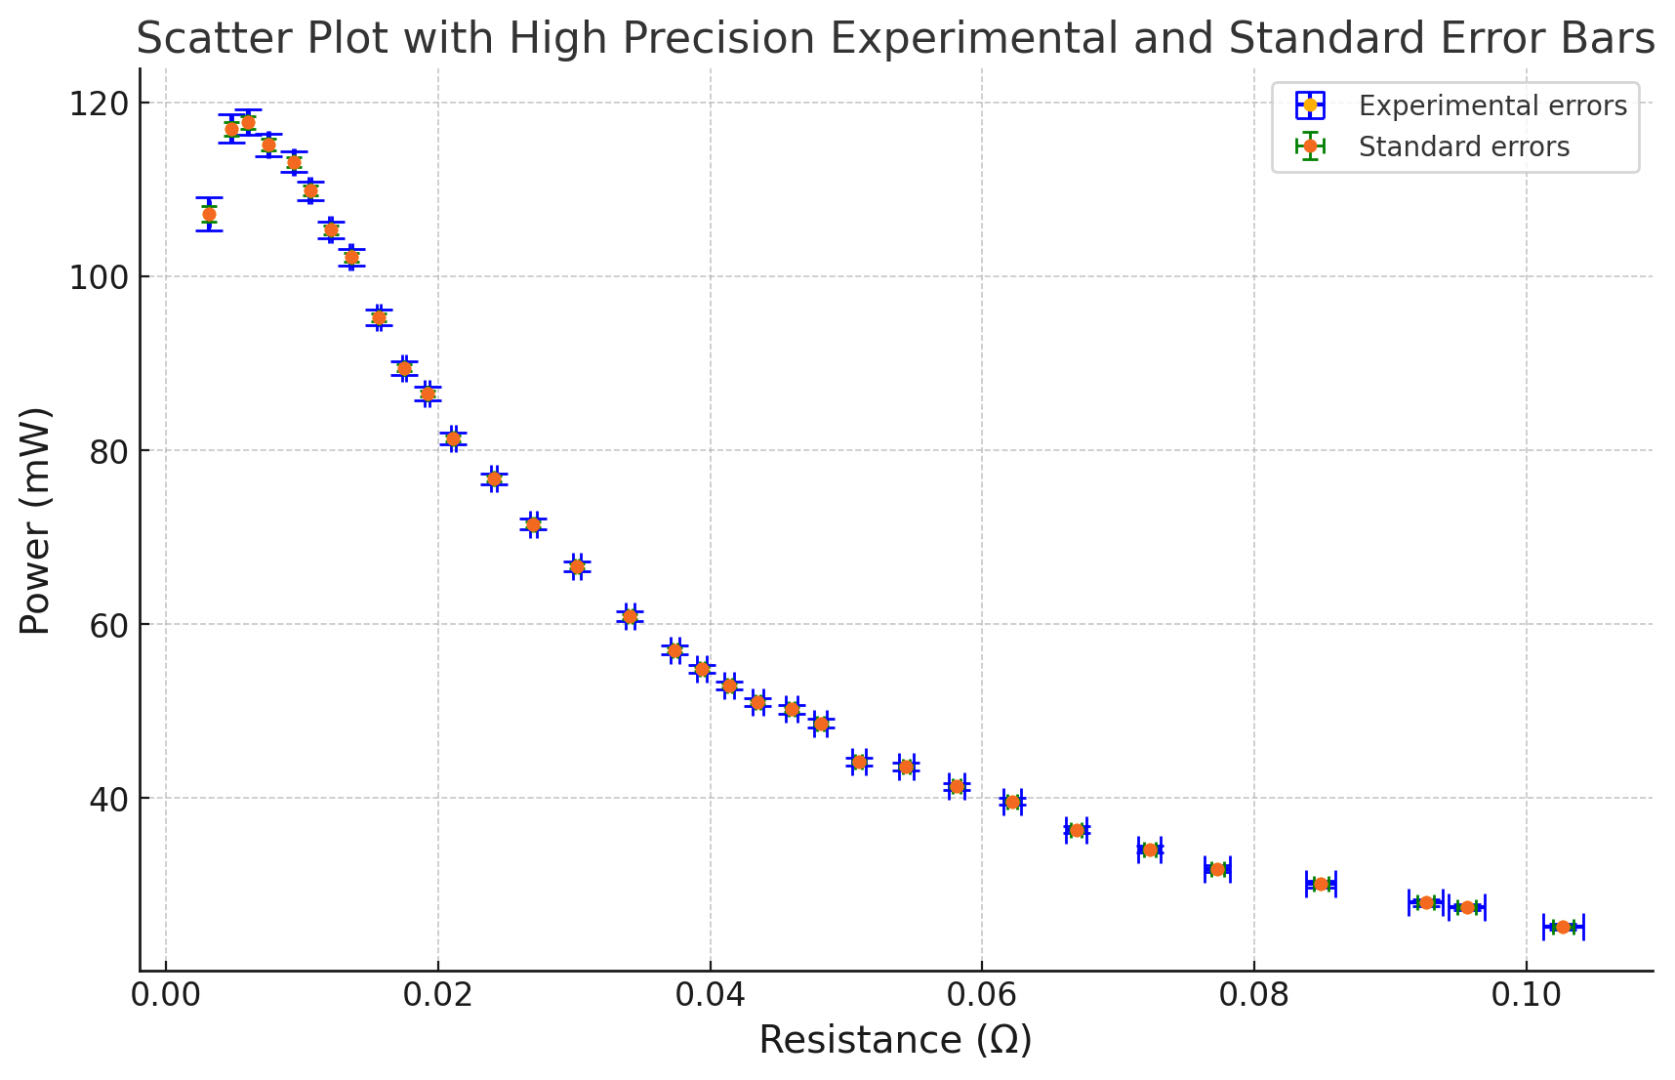
\includegraphics[width=0.47\textwidth]{并联电压耦合P-R+误差棒.jpg}\label{fig:并联电压耦合P-R+误差棒}}
                    \caption{双TEC片并联电压耦合数据处理+误差棒绘制}
                    \label{fig:双TEC片并联电压耦合数据处理}
                \end{figure}


               


        \end{enumerate}




        \begin{table}[htbp]
            \centering
            \small
            \begin{minipage}{0.45\textwidth}
                \centering
                \begin{tblr}{
                    vline{1,3,5} = {-}{},
                    hline{1-2,35} = {-}{},
                }
                $U/V$ & $I/mA$ & $P/mW$ & $R_L/\Omega$ \\
                1.61 & 15.68 & 25.16 & 204.87 \\
                1.62 & 16.95 & 27.48 & 191.40 \\
                1.61 & 17.39 & 27.99 & 184.49 \\
                1.60 & 18.84 & 30.04 & 169.97 \\
                1.57 & 20.30 & 31.94 & 155.56 \\
                1.57 & 21.73 & 34.10 & 144.21 \\
                1.56 & 23.31 & 36.26 & 133.64 \\
                1.57 & 25.25 & 39.67 & 124.70 \\
                1.55 & 26.67 & 41.24 & 116.25 \\
                1.54 & 28.31 & 43.60 & 108.96 \\
                1.50 & 29.45 & 44.15 & 102.32 \\
                1.53 & 31.78 & 48.55 & 96.30 \\
                1.52 & 33.03 & 50.24 & 91.14 \\
                1.49 & 34.25 & 50.85 & 86.29 \\
                1.48 & 35.79 & 52.81 & 82.40 \\
                1.47 & 37.32 & 54.68 & 78.12 \\
                1.46 & 39.06 & 56.87 & 74.90 \\
                1.44 & 42.29 & 60.71 & 68.35 \\
                1.42 & 46.95 & 66.45 & 60.12 \\
                1.39 & 51.43 & 71.21 & 53.92 \\
                1.36 & 56.40 & 76.40 & 48.21 \\
                1.31 & 62.10 & 81.37 & 42.32 \\
                1.29 & 67.06 & 86.28 & 38.56 \\
                1.25 & 71.58 & 89.43 & 34.89 \\
                1.22 & 78.09 & 94.98 & 31.07 \\
                1.18 & 86.59 & 102.43 & 27.23 \\
                1.13 & 93.20 & 105.26 & 24.16 \\
                1.08 & 101.69 & 110.22 & 21.25 \\
                1.03 & 109.84 & 113.37 & 18.82 \\
                0.93 & 123.79 & 114.65 & 15.02 \\
                0.84 & 140.13 & 117.39 & 12.06 \\
                0.75 & 155.96 & 116.55 & 9.51 \\
                0.58 & 184.75 & 106.78 & 6.27 \\
                \end{tblr}
                \caption{串联的外输出特性}
                \label{tbl:串联的外输出特性}
            \end{minipage}
            \hfill
            \begin{minipage}{0.45\textwidth}
                \centering
                \begin{tblr}{
                    vline{1,3,5} = {-}{},
                    hline{1-2,35} = {-}{},
                }
                $U/V$ & $I/mA$ & $P/mW$ & $R_L/\Omega$ \\
                1.0294 & 17.973 & 18.502 & 57.274 \\
                1.0249 & 19.249 & 19.73 & 53.246 \\
                1.0233 & 19.903 & 20.366 & 51.415 \\
                1.0184 & 21.486 & 21.88 & 47.397 \\
                1.014 & 23.27 & 23.595 & 43.575 \\
                1.0098 & 24.976 & 25.222 & 40.432 \\
                1.0035 & 26.762 & 26.855 & 37.496 \\
                0.997 & 28.739 & 28.653 & 34.691 \\
                0.9868 & 30.429 & 30.026 & 32.429 \\
                0.9794 & 32.241 & 31.577 & 30.377 \\
                0.9697 & 33.792 & 32.769 & 28.697 \\
                0.9651 & 36.024 & 34.766 & 26.79 \\
                0.9598 & 37.73 & 36.212 & 25.438 \\
                0.9512 & 39.289 & 37.372 & 24.21 \\
                0.9482 & 41.041 & 38.916 & 23.104 \\
                0.9399 & 42.879 & 40.302 & 21.919 \\
                0.936 & 44.688 & 41.827 & 20.945 \\
                0.9204 & 48.308 & 44.463 & 19.053 \\
                0.9038 & 53.731 & 48.56 & 16.82 \\
                0.8895 & 58.95 & 52.434 & 15.088 \\
                0.8667 & 64.538 & 55.932 & 13.428 \\
                0.8451 & 71.276 & 60.237 & 11.857 \\
                0.8279 & 76.791 & 63.573 & 10.781 \\
                0.8001 & 81.967 & 65.584 & 9.762 \\
                0.7766 & 89.367 & 69.401 & 8.69 \\
                0.7499 & 98.782 & 74.075 & 7.591 \\
                0.7239 & 106.79 & 77.305 & 6.779 \\
                0.6908 & 116.279 & 80.32 & 5.94 \\
                0.6588 & 125.519 & 82.691 & 5.249 \\
                0.5984 & 142.029 & 84.987 & 4.213 \\
                0.5375 & 160.129 & 86.068 & 3.357 \\
                0.4781 & 178.876 & 85.521 & 2.673 \\
                0.3728 & 212.01 & 79.042 & 1.759 \\
                \end{tblr}
                \caption{并联的外输出特性}
                \label{tbl:并联的外输出特性}
            \end{minipage}
        \end{table}

    \subsection{基于热力学建模的散热修正}
    
        我们基于简单的热力学建模,编写Python脚本模拟了置于保温材料中的热机热端(假设为一个小圆点)在开始加热后的升温情况,如\cref{fig:热力学建模的散热修正图1}所示。

        \begin{figure}[htbp]
            \centering
            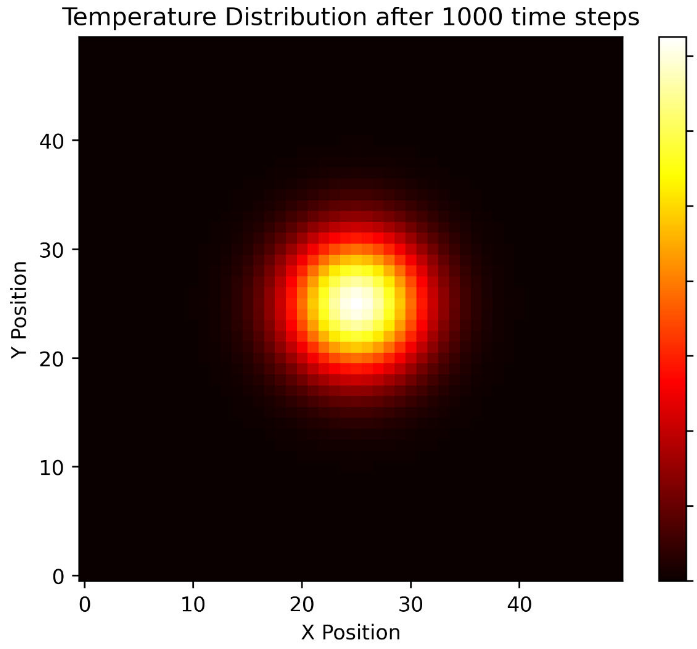
\includegraphics[width=0.6\textwidth]{热力学建模的散热修正图1.png}
            \caption{热力学建模的散热修正}
            \label{fig:热力学建模的散热修正图1}
        \end{figure}
    
        接下来我们基于一些热力学定律,简单建模计算了散热功率。

        假设参数:热机的表面积 \( A \) 假定为 0.01 平方米。
        对流换热系数 \( h \) 假定为 10 W/(m²·K)。
        热机表面的发射率 \( \epsilon \) 假定为 0.9。
        Stefan-Boltzmann常数 \( \sigma \approx 5.67 \times 10^{-8} \) W/(m²·K⁴)。
        环境温度 \( T_{\text{ambient}} = 30 \) °C(303 K)。
        热机核心温度 \( T_{\text{surface}} = 48 \) °C(321 K)。
        外界输入总功率为 8 瓦特。

                计算通过对流损失的热量:
        \[
        Q_{\text{conv}} = 10 \times 0.01 \times (321 - 303) = 1.8 \text{ W}
        \]

        计算通过辐射损失的热量:
        \[
        Q_{\text{rad}} = 0.9 \times 5.67 \times 10^{-8} \times 0.01 \times (321^4 - 303^4)
        \]

        总的热损失:
        \[
        Q_{\text{total}} = Q_{\text{conv}} + Q_{\text{rad}}
        \]

        计算表面温度和环境温度的四次方:

        \[ T_{\text{surface}}^4 = 321^4 = 10510137681 \]
        \[ T_{\text{ambient}}^4 = 303^4 = 8419395361 \]

        计算辐射热损失:

        \[ Q_{\text{rad}} = 0.9 \times 5.67 \times 10^{-8} \times 0.01 \times (10510137681 - 8419395361) \]
        \[ Q_{\text{rad}} = 0.9 \times 5.67 \times 10^{-8} \times 0.01 \times 2090742319.86 \]
        \[ Q_{\text{rad}} = 0.9 \times 1.186376896 \]
        \[ Q_{\text{rad}} = 1.0677392064 \text{ W} \]


        总的热损失:

        \[ Q_{\text{total}} = Q_{\text{conv}} + Q_{\text{rad}} \]
        \[ Q_{\text{total}} = 1.8 + 1.0677392064 \]
        \[ Q_{\text{total}} = 2.8677392064 \text{ W} \]

        对流热损失: \( Q_{\text{conv}} = 1.8 \) W

        辐射热损失: \( Q_{\text{rad}} = 1.0677 \) W

        总的热损失: \( Q_{\text{total}} = 2.8677 \) W

        则可计算出热机效率$ \eta = \frac{P_{out}}{P_{in} - Q_{total}} = \frac{0.0485}{8.568 - 2.8677} = 0.7\% $

        而该温差下的卡诺热机效率为37.5\%。



\clearpage
\section{总结及存在问题}

    \begin{itemize}
        \item 总结:
        
            \begin{enumerate}
                \item 热电效应的验证:通过实验,我们成功验证了Seebeck效应,测量了不同温差下的开路电压,并计算了Seebeck系数。这些结果与理论值基本一致,说明我们的实验装置和测量方法是可靠的。
                
                \item 热电发电装置的性能分析:我们测量了热电发电装置在不同负载下的输出特性,发现最大输出功率出现在负载电阻等于内阻时。通过优化热源和冷源的温度,提高了热电发电装置的输出性能。
                
                \item 热电堆的优化:我们探索了不同热电模块的耦合方式,包括串联和并联,发现合适的耦合方式可以显著提高输出电压和电流,从而提高输出功率。
                
                \item 散热特性的建模分析:通过热力学建模和实验数据,我们分析了热机的散热特性,发现对流和辐射散热是主要的热损失途径。通过使用高效的隔热材料和优化冷却系统,可以减少热损失,提高热机效率。
                
                \item 热机效率的验证:在优化温差和减少热损失的情况下,我们测量了热机的效率,并与卡诺热机的理论效率进行了比较。尽管实验热机的效率远低于卡诺热机效率,但仍验证了热力学第二定律的正确性。
            \end{enumerate}


        \item 存在的问题
        
            \begin{enumerate}
                \item 测量误差:在温度测量和电压电流测量过程中,存在一定的误差。这些误差主要来源于测量设备的精度和环境因素的影响。例如,PT100温度传感器的精度和电压表、电流表的测量误差都对实验结果有影响。未来实验中,可以通过使用更高精度的测量设备和改进实验环境来减少误差。

                \item 散热问题:实验过程中,热机的散热问题较为明显,特别是在高温差条件下,对流和辐射散热导致了显著的热损失,影响了热机的效率。未来可以考虑采用更高效的隔热材料和冷却技术来减少散热损失。
                
                \item 热电材料的性能:热电材料的性能对热机的输出功率和效率有直接影响。目前使用的热电材料转换效率较低,限制了热电发电装置的应用范围。未来可以通过材料科学的进步,研发更高效的热电材料,提高能量转换效率。
                
                \item 实验装置的优化:实验装置的设计和搭建对实验结果有重要影响。虽然本次实验中,我们搭建了基本的热电发电装置,但仍有很多优化空间。例如,热电模块的排列方式、冷却系统的设计、负载匹配等,都可以进一步优化,以提高实验装置的性能。
            \end{enumerate}
    \end{itemize}


    总的来说,本实验验证了热电效应在热机设计中的应用潜力,但也暴露了若干问题。通过改进测量方法、优化实验装置和研发更高效的热电材料,可以进一步提高基于热电效应的热机效率,为实际应用提供更多可能性。






\clearpage
\section{附录}


    % 设置Python代码的样式
    \lstset{
        language=Python, % 设置语言为Python
        basicstyle=\ttfamily, % 使用等宽字体
        keywordstyle=\color{blue}\bfseries, % 关键字样式为蓝色粗体
        commentstyle=\color{green!60!black}, % 注释样式为深绿色
        stringstyle=\color{red}, % 字符串样式为红色
        showstringspaces=false, % 不显示字符串中的空格
        frame=single, % 设置代码框
        breaklines=true, % 自动换行
        numbers=left, % 行号显示在左侧
        numberstyle=\small\ttfamily\color{gray}, % 行号样式
        captionpos=b % 标题位置
    }


    





    热力学模拟python代码:

    \begin{lstlisting}
        import numpy as np
        import matplotlib.pyplot as plt
        
        # Simulation parameters
        nx, ny = 50, 50  # Number of grid points
        dx = dy = 1.0  # Distance between grid points
        alpha = 0.01  # Thermal diffusivity
        dt = 0.1  # Time step
        num_steps = 10000  # Number of time steps
        
        # Initial temperature distribution
        T = np.ones((nx, ny)) * 303  # Ambient temperature 30°C in Kelvin
        
        # Heat source at the center
        source_x, source_y = nx // 2, ny // 2
        T[source_x, source_y] = 321  # Heat source temperature 48°C in Kelvin
        
        # Simulation function
        def update(T, alpha, dt, dx, dy):
            T_new = T.copy()
            for i in range(1, nx-1):
                for j in range(1, ny-1):
                    T_new[i, j] = T[i, j] + alpha * dt * (
                        (T[i+1, j] - 2*T[i, j] + T[i-1, j]) / dx**2 +
                        (T[i, j+1] - 2*T[i, j] + T[i, j-1]) / dy**2
                    )
            return T_new
        
        # Run the simulation for the specified number of steps
        for _ in range(num_steps):
            T = update(T, alpha, dt, dx, dy)
        
        # Plot the final temperature distribution
        plt.figure(figsize=(8, 6))
        plt.imshow(T, cmap='hot', origin='lower')
        plt.colorbar(label='Temperature (K)')
        plt.title('Temperature Distribution after 1000 time steps')
        plt.xlabel('X Position')
        plt.ylabel('Y Position')
        plt.show()
    \end{lstlisting}

    \begin{thebibliography}{99}

        \bibitem{Boltzmann1877}
        Boltzmann, L. (1877). ``Über die Beziehung zwischen dem zweiten Hauptsatze der mechanischen Wärmetheorie und der Wahrscheinlichkeitsrechnung respektive den Sätzen über das Wärmegleichgewicht.'' \emph{Wiener Berichte}, 76, 373-435.
        
        \bibitem{Carnot1824}
        Carnot, S. (1824). \emph{Réflexions sur la puissance motrice du feu et sur les machines propres à développer cette puissance.} Bachelier, Paris.
        
        \bibitem{WalshFletcher2004}
        Walsh, P. P., \& Fletcher, P. (2004). \emph{Gas Turbine Performance.} Blackwell Science.
        
        \bibitem{Goldsmid2010}
        Goldsmid, H. J. (2010). \emph{Introduction to Thermoelectricity.} Springer Series in Materials Science, 121.
        
    \end{thebibliography}

\end{document}
